\باب{درجہ دوم سادہ تفرقی مساوات}
کئی اہم میکانی اور برقی مسائل کو خطی دو درجی تفرقی مساوات سے ظاہر کیا جا سکتا ہے۔خطی دو درجی تفرقی مساوات  تمام خطی تفرقی مساوات کی نمائندگی کرتا ہے۔چونکہ دو درجی مساوات کا حل نسبتاً آسان ہوتا ہے لہٰذا اس باب میں اسی پر پہلے غور کرتے ہیں۔اگلے باب کا موضوع تین درجی مساوات ہے۔

تفرقی مساوات کو خطی اور غیر خطی گروہوں میں تقسیم کیا جاتا ہے۔غیر خطی تفرقی مساوات کے حل کا حصول مشکل ثابت ہوتا ہے جبکہ خطی مساوات حل کرنے کے کئی عمدہ ترکیب پائے جاتے ہیں۔اس باب میں عمومی حل اور ابتدائی معلومات کی صورت میں مخصوص حل کا حصول دکھایا جائے گا۔

\حصہ{متجانس خطی دو درجی تفرقی مساوات}
یک درجی مساوات پر پہلے باب میں غور کیا گیا۔اس باب میں دو درجی مساوات پر غور کیا جائے گا۔یہ مساوات میکانی اور برقی \اصطلاح{ارتعاش}\فرہنگ{ارتعاش}\حاشیہب{oscillations}\فرہنگ{oscillations}، متحرک امواج، منتقلی حرارتی توانائی اور طبیعیات کے دیگر شعبوں میں کلیدی کردار ادا کرتے ہیں۔

ایسا دو درجی تفرقی مساوات جس کو
\begin{align}\label{مساوات_سادہ_دو_درجی_تعریف}
y''+p(x)y'+q(x)y=r(x)
\end{align}
صورت میں لکھا جا سکے \اصطلاح{خطی}\فرہنگ{خطی!دو درجی}\حاشیہب{linear}\فرہنگ{linear!second order} کہلاتا ہے ورنہ اس کو \اصطلاح{غیر خطی}\فرہنگ{غیر خطی}\حاشیہب{nonlinear}\فرہنگ{nonlinear} کہتے ہیں۔

اس مساوات کی خاصیت یہ ہے کہ اس میں \عددی{y}، \عددی{y'} اور \عددی{y''} کی طاقت اکائی ہے  یعنی تینوں خطی ہیں البتہ \عددی{p(x)}، \عددی{q(x)} اور \عددی{r(x)} متغیرہ \عددی{x} کے کوئی بھی تفاعل ہو سکتے ہیں۔دو درجی مساوات کا پہلا جزو \عددی{f(x)y''} ہونے کی صورت میں مساوات کو \عددی{f(x)} سے تقسیم کرتے ہوئے اس کو مساوات \حوالہ{مساوات_سادہ_دو_درجی_تعریف} کی \اصطلاح{معیاری صورت}\فرہنگ{معیاری صورت!دو درجی}\حاشیہب{standard form}\فرہنگ{standard form!second order} میں لکھیں جہاں  \عددی{y''} پہلا  جزو ہے۔

متجانس اور غیر متجانس دو درجی مساوات کی تعریف ہو بہو ایک درجی متجانس اور غیر متجانس مساوات کی تعریف کی طرح ہے جس پر حصہ \حوالہ{حصہ_سادہ_اول_متجانس_خطی} میں تبصرہ کیا گیا۔یقیناً \عددی{r \equiv 0} [جہاں زیر غور تمام \عددی{x} پر  \عددی{r(x)=0} ہو؛ اس کو \اصطلاح{مکمل صفر}\فرہنگ{مکمل صفر}\حاشیہب{identically zero}\فرہنگ{identically zero} پڑھیں۔] کی صورت میں مساوات \حوالہ{مساوات_سادہ_دو_درجی_تعریف} درج ذیل لکھی جائے گی 
\begin{align}\label{مساوات_سادہ_متجانس_دو_درجی_تعریف}
y''+p(x)y'+q(x)y=0
\end{align}
جو \اصطلاح{متجانس} ہے۔اگر \عددی{r(x) \not\equiv 0} ہو تب مساوات \حوالہ{مساوات_سادہ_دو_درجی_تعریف} \اصطلاح{غیر متجانس}\فرہنگ{غیر متجانس!دو درجی}\حاشیہب{nonhomogenous}\فرہنگ{nonhomogenous!second order} کہلائے گا۔

متجانس خطی تفرقی مساوات کی مثال درج ذیل ہے
\begin{align*}
xy''+2y'+y=0,\quad \text{\RL{ جو کو معیاری صورت میں لکھتے ہیں}} \quad y''+\frac{2y'}{x}+\frac{y}{x}=0
\end{align*}
جبکہ غیر متجانس خطی تفرقی مساوات کی مثال
\begin{align*}
y''+x^2y=\sec x
\end{align*}
ہے۔آخر میں غیر خطی مساوات کی تین مثال پیش کرتے ہیں۔
\begin{align*}
\left(y''\right)^3+xy=\sin x, \quad y''+xy'+4y^2=0, \quad yy''-xy'=0
\end{align*}
تفاعل \عددی{p} اور \عددی{q} مساوات \حوالہ{مساوات_سادہ_متجانس_دو_درجی_تعریف} کے \اصطلاح{عددی سر}\فرہنگ{عددی سر!دو درجی مساوات}\حاشیہب{coefficients}\فرہنگ{coefficients} کہلاتے ہیں۔

دو درجی مساوات کے حل کی تعریف عین ایک درجی مساوات کے حل کی مانند ہے۔ تفاعل \عددی{y=h(x)} کو کھلے وقفہ \عددی{I} پر اس صورت خطی (یا غیر خطی) دو درجی تفرقی مساوات کا حل تصور کیا جاتا ہے جب اس پورے فاصلے پر \عددی{h(x)}، \عددی{h'} اور \عددی{h''}  پائے جاتے ہوں اور  تفرقی مساوات میں \عددی{y} کی جگہ \عددی{h}، \عددی{y'} کی جگہ \عددی{h'} اور \عددی{y''} کی جگہ \عددی{h''} پر کرنے سے مساوات کے دونوں اطراف بالکل یکساں صورت اختیار کرتے ہوں۔چند مثال جلد پیش کرتے ہیں۔
%==========================

\حصہء{متجانس خطی تفرقی مساوات}
اس باب کے پہلے حصے میں متجانس خطی مساوات پر غور کیا جائے گا جبکہ بقایا باب میں غیر متجانس خطی مساوات پر غور کیا جائے گا۔ 

خطی تفرقی مساوات حل کرنے کے نہایت عمدہ تراکیب پائے جاتے ہیں۔متجانس مساوات کے حل میں \اصطلاح{اصول خطیت}\فرہنگ{اصول!خطیت}\فرہنگ{خطیت!اصول}\حاشیہب{linearity principle}\فرہنگ{linearity!principle} یا \اصطلاح{اصول نفاذ}\فرہنگ{اصول!نفاذ}\فرہنگ{نفاذ!اصول}\حاشیہب{superposition principle}\فرہنگ{superposition!principle} کلیدی کردار ادا کرتا ہے جس کے تحت متجانس مساوات کے مختلف حل کو آپس میں جمع کرنے یا انہیں مستقل سے ضرب دینے سے دیگر حل حاصل کئے جا سکتے ہیں۔
%===================

\ابتدا{مثال}\شناخت{مثال_سادہ_دو_درجی_اصول_نفاذ}\quad اصول نفاذ\\
تمام \عددی{x} پر درج ذیل متجانس خطی تفرقی مساوات کے حل \عددی{y_1=\cos 2x} اور \عددی{y_2=\sin 2x} ہیں۔
\begin{align}
y''+4y=0
\end{align}
ان حل کی درستگی ثابت کرنے کی خاطر انہیں دیے گئے مساوات میں پر کرتے ہیں۔پہلے \عددی{y_1=\cos 2x} کو درست حل ثابت کرتے ہیں۔چونکہ \عددی{(\cos 2x)''=-4\cos 2x} کے برابر ہے لہٰذا 
\begin{align*}
y''+4y=(\cos 2x)''+4(\cos 2x)=-4\cos 2x+4\cos 2x=0
\end{align*}
ملتا ہے۔اسی طرح \عددی{y_2=\sin 2x} کو پر کرتے ہوئے 
\begin{align*}
y''+4y=(\sin 2x)''+4(\sin 2x)=-4\sin 2x+4\sin 2x=0
\end{align*}
ملتا ہے۔ہم دیے گئے حل سے نئے حل حاصل کر سکتے ہیں۔یوں ہم \عددی{\cos 2x} کو کسی مستقل مثلاً \عددی{2.73} سے ضرب دیتے ہوئے اور \عددی{\sin 2x} کو  \عددی{-1.25} سے ضرب دیتے ہوئے ان کا مجموعہ
\begin{align*}
y_3=2.73\cos 2x-1.25\sin 2x
\end{align*}
لیتے ہوئے  توقع کرتے ہیں کہ یہ بھی دیے گئے تفرقی مساوات کا حل ہو گا۔آئیں نئے حل کو تفرقی مساوات میں پر کرتے ہوئے اس کی درستگی ثابت کریں۔
\begin{align*}
y''+4y&=(2.73\cos 2x-1.25\sin 2x)''+4(2.73\cos 2x-1.25\sin 2x)\\
&=4(-2.73\cos 2x+1.25\sin 2x)+4(2.73\cos 2x-1.25\sin 2x)\\
&=0
\end{align*}
\انتہا{مثال}
%=======================

اس مثال میں ہم نے دیے گئے حل \عددی{y_1} اور \عددی{y_2} سے نیا حل 
\begin{align}
y_3=c_1 y_1+c_2 y_2, \quad \text{\RL{($c_1$\, اور \, $c_2$\,اختیاری مستقل ہیں)}}
\end{align}
حاصل کیا۔ اس کو \عددی{y_1} اور \عددی{y_2} کا \اصطلاح{خطی میل}\فرہنگ{خطی!میل}\حاشیہب{linear combination}\فرہنگ{linear!combination} کہتے ہیں۔اس مثال سے ہم \اصطلاح{مسئلہ خطی میل}\فرہنگ{مسئلہ!خطی میل} بیان کرتے ہیں جسے عموماً \اصطلاح{اصول خطیت}\فرہنگ{اصول!خطیت} یا \اصطلاح{اصول نفاذ}\فرہنگ{اصول نفاذ} کہا جاتا ہے۔

%======================================

\ابتدا{مسئلہ}\شناخت{مسئلہ_دو_درجی_خطی_میل}\quad مسئلہ خطی میل\\
کھلے وقفہ \عددیء{I} پر متجانس خطی دو درجی تفرقی مساوات کے دو عدد حل کا خطی میل بھی \عددیء{I} پر اس مساوات کا حل ہو گا۔بالخصوص ان حل کو مستقل مقدار سے ضرب دینے سے بھی مساوات کے حل حاصل ہوتے ہیں۔
\انتہا{مسئلہ}

ثبوت: تصور کریں کہ متجانس مساوات \حوالہ{مساوات_سادہ_متجانس_دو_درجی_تعریف} کے دو حل \عددی{y_1} اور \عددی{y_2} پائے جاتے ہیں لہٰذا
\begin{gather}
\begin{aligned}\label{مساوات_درجہ_دو_خطی_میل}
y_1''+py_1'+qy_1&=0\\
y_2''+y_2'+qy_2&=0
\end{aligned}
\end{gather}
ہو گا۔خطی میل سے نیا حل \عددی{y_3=c_1 y_1+c_2 y_2} حاصل کرتے ہیں۔اس کا ایک درجی تفرق اور دو درجی تفرق درج ذیل ہیں۔
\begin{align*}
y_3' &=c_1y_1'+c_2y_2'\\
y_3'' &=c_1 y_1''+c_2y_2''
\end{align*}
\عددی{y_3}، \عددی{y_3'} اور \عددی{y_3''} کو متجانس مساوات کے بائیں ہاتھ میں پر کرتے ہیں
\begin{align*}
y_3''+py_3'+qy_3&=(c_1 y_1''+c_2y_2'')+p(c_1y_1'+c_2y_2')+q(c_1 y_1+c_2 y_2)\\
&=c_1(y_1''+py_1'+qy_1)+c_2(y_2''+py_2'+qy_2)\\
&=0
\end{align*}
جہاں مساوات \حوالہ{مساوات_درجہ_دو_خطی_میل} سے آخری قدم پر دونوں قوسین صفر کے برابر پر کئے گئے ہیں۔یوں مساوات کا بایاں ہاتھ اور دایاں ہاتھ برابر ہیں لہٰذا ثابت ہوتا ہے کہ \عددی{y_3} بھی مساوات   \حوالہ{مساوات_سادہ_متجانس_دو_درجی_تعریف} کا حل ہے۔

یہاں یاد رہے کہ مسئلہ \حوالہ{مسئلہ_دو_درجی_خطی_میل} صرف متجانس مساوات کے لئے قابل استعمال ہے۔غیر متجانس مساوات کے دیگر حل اس مسئلے سے حاصل نہیں کئے جا سکتے ہیں۔
%======================================

\ابتدا{مثال}
تصور کریں کہ \عددی{y_1} اور \عددی{y_2} غیر متجانس مساوات \حوالہ{مساوات_سادہ_دو_درجی_تعریف} کے حل ہیں۔ثابت کریں کہ \عددی{y_3=c_1y_1+c_2y_2} اس متجانس مساوات کا حل نہیں ہے جہاں \عددی{c_1} اور \عددی{c_2} مستقل مقدار ہیں۔

حل:\عددی{y_1} اور \عددی{y_2} غیر متجانس مساوات کے حل ہیں لہٰذا انہیں متجانس مساوات میں پر کرنے سے مساوات کے دونوں اطراف برابر حاصل ہوتے ہیں یعنی
\begin{gather}
\begin{aligned}\label{مساوات_سادہ_دو_درجی_غیر_متجانس_حل_الف}
y_1''+py_1'+qy_1&=r\\
y_2''+py_2'+qy_2&=r
\end{aligned}
\end{gather}
\عددی{y_3} کو مساوات کے بائیں ہاتھ میں پر کرتے ہیں
\begin{align*}
y_3''+py'+qy&=(c_1y_1+c_2y_2)''+p(c_1y_1+c_2y_2)'+q(c_1y_1+c_2y_2)\\
&=(c_1y_1''+c_2y_2'')+p(c_1y_1'+c_2y_2')+q(c_1y_1+c_2y_2)\\
&=c_1(y_1''+py_1'+qy_1)+c_2(y_2''+py_2'+qy_2)\\
&=(c_1+c_2)r
\end{align*}
 جہاں آخری قدم پر مساوات \حوالہ{مساوات_سادہ_دو_درجی_غیر_متجانس_حل_الف} کا استعمال کیا گیا۔اس سے \عددی{(c_1+c_2)r} حاصل ہوتا ہے جبکہ متجانس مساوات کا دایاں ہاتھ \عددی{r} کے برابر ہے لہٰذا \عددی{y_3} متجانس مساوات پر پورا نہیں اترتا۔یوں \عددی{y_3} متجانس مساوات کا حل نہیں ہے۔
\انتہا{مثال}
%=====================================
\ابتدا{مشق}\quad غیر متجانس خطی مساوات\\
درج ذیل خطی غیر متجانس مساوات میں \عددی{y=2-\cos x} اور \عددی{y=2-\sin x} کو پر کرتے ہوئے ثابت کریں کہ یہ مساوات کے حل ہیں۔ثابت کریں کہ ان کا مجموعہ مساوات کا حل نہیں ہے۔اسی طرح ثابت کریں کہ \عددی{3(2-\cos x)} یا \عددی{-7(2-\sin x)} بھی مساوات کے حل نہیں ہیں۔
\begin{align*}
y''+y=2
\end{align*}

\انتہا{مشق}
%==================================
\ابتدا{مشق}
درج ذیل مساوات میں \عددی{y=1} اور \عددی{y=x^3} پر کرتے ہوئے ثابت کریں کہ یہ دونوں تفرقی مساوات کے حل ہیں۔ثابت کریں کہ ان کا مجموعہ تفرقی مساوات کا حل نہیں ہے نا ہی \عددی{y=-x^3} حل ہے۔اس کا مطلب یہ ہوا کہ حل کو \عددی{-1} سے بھی ضرب دے کر نیا حل نہیں حاصل کیا جا سکتا ہے۔
\begin{align*}
yy''-2x^2y'=0
\end{align*}
\انتہا{مشق}
%=================================

\حصہء{ابتدائی قیمت مسائل۔ اساس۔ عمومی حل}
باب \حوالہ{باب_سادہ_اول_تفرقی} میں ابتدائی قیمت درجہ اول سادہ تفرقی مساوات پر غور کیا گیا۔درجہ اول سادہ تفرقی مساوات اور ابتدائی معلومات \عددی{y(x_0)=y_0} مل کر ابتدائی قیمت تفرقی مساوات کہلاتے ہیں۔ابتدائی قیمت کو استعمال کرتے ہوئے درجہ اول سادہ تفرقی مساوات کے عمومی حل کا واحد اختیاری مستقل \عددی{c} حاصل کرتے ہوئے مخصوص یکتا حل حاصل کیا جاتا ہے۔اسی تصور کو دو درجی سادہ تفرقی مساوات تک بڑھاتے ہیں۔

دو درجی متجانس خطی ابتدائی قیمت مسئلے سے مراد متجانس مساوات \حوالہ{مساوات_سادہ_متجانس_دو_درجی_تعریف} اور درج ذیل ابتدائی معلومات ہیں۔
\begin{align}\label{مساوات_سادہ_دو_درجی_ابتدائی_قیمتیں}
y(x_0)=K_0,\quad y'(x_0)=K_1
\end{align}
\عددی{K_0} اور \عددی{K_1}  کھلے وقفہ پر نقطہ \عددی{x_0} پر بالترتیب نقطہ عمومی حل اور حل کے تفرق (یعنی ڈھلوان) کی قیمتیں ہیں۔ 

مساوات \حوالہ{مساوات_سادہ_دو_درجی_ابتدائی_قیمتیں} میں دیے گئے ابتدائی قیمتوں سے عمومی حل
\begin{align}
y=c_1y_1+c_2y_2
\end{align}
کے اختیاری مستقل \عددی{c_1} اور \عددی{c_2} کی قیمتیں حاصل کی جاتی ہیں۔یہاں \عددی{y_1} اور \عددی{y_2} مساوات \حوالہ{مساوات_سادہ_دو_درجی_ابتدائی_قیمتیں} کے حل ہیں۔یوں مخصوص حل حاصل کیا جاتا ہے جو نقطہ \عددی{(x_0,K_0)} سے گزرتا ہے اور جس کی ڈھلوان اس نقطے پر \عددی{K_1} ہوتی ہے۔
%==============

\ابتدا{مثال}\شناخت{مثال_سادہ_دو_درجی_ابتدائی_قیمت_الف}
درج ذیل ابتدائی قیمت دو درجی سادہ تفرقی مساوات کو حل کریں۔
\begin{align*}
y''+4y=0,\quad y(0)=5,\quad y'(0)=-3
\end{align*}

حل:پہلا قدم: اس مساوات کے حل  \عددی{y_1=\cos 2x} اور \عددی{y_2=\sin 2x} ہیں (مثال \حوالہ{مثال_سادہ_دو_درجی_اصول_نفاذ} سے رجوع کریں) لہٰذا اس کا موزوں عمومی حل
\begin{align}\label{مساوات_سادہ_دو_درجی_عمومی_حل_الف}
y=c_1\cos 2x+c_2\sin 2x
\end{align}
ہو گا۔ (موزوں حل پر اس مثال کے فوراً بعد بات کرتے ہیں۔)

دوسرا قدم:مخصوص حل حاصل کرتے ہیں۔عمومی حل کا تفرق \عددی{y'=-2\sin 2x +2c_2\cos x} ہے۔ابتدائی قیمتیں استعمال کرتے ہوئے
\begin{align*}
y(0)&=c_1 \cos 0+c_2\sin 0=c_1=5\\
y'(0)&=-2\sin 0+2c_2\cos 0=2c_2=-3, \quad c_2=-1.5
\end{align*}
حاصل ہوتے ہیں لہٰذا مخصوص حل
\begin{align*}
y=5\cos 2x-1.5\sin 2x
\end{align*}
ہو گا۔شکل \حوالہ{شکل_مثال_سادہ_دو_درجی_ابتدائی_قیمت_الف} میں مخصوص حل دکھایا گیا ہے۔نقطہ \عددی{x=0} پر اس کی قیمت \عددی{y(0)=5} ہے جبکہ اسی نقطے پر خط کی ڈھلوان (مماس) \عددی{y'(0)=0.5} ہے۔مماس \عددی{x} محور کو \عددی{x=\tfrac{5}{3}=3.33} پر قطع کرتا ہے۔
\begin{figure}
\centering
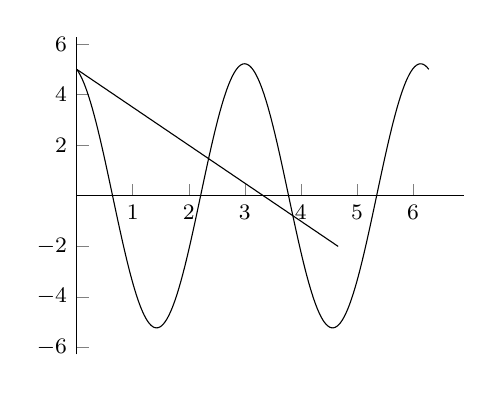
\begin{tikzpicture}
\begin{axis}[small,axis lines*=middle,xmin=0]
\addplot[domain=0:2*pi,samples=200]{5*cos(2*x*180/pi)-1.5*sin(2*x*180/pi)};
\addplot[] plot coordinates {(0,5) (4.666,-2)};
\end{axis}
\end{tikzpicture}
\caption{مثال \حوالہ{مثال_سادہ_دو_درجی_ابتدائی_قیمت_الف} کا مخصوص حل۔}
\label{شکل_مثال_سادہ_دو_درجی_ابتدائی_قیمت_الف}
\end{figure}
\انتہا{مثال}
%===================

درج بالا مثال میں \عددی{y_1} اور \عددی{y_2} ایسے تفاعل تھے جن سے حاصل عمومی حل ابتدائی معلومات پر پورا اترتا تھا۔آئیں اب دو آپس میں راست تناسب حل لیتے ہوئے عمومی حل  لکھیں، مثلاً \عددی{y_1=\cos 2x} اور \عددی{y_2=k\cos 2x} لیتے ہوئے
\begin{align*}
y=c_1\cos 2x+c_2 k\cos 2x=(c_1+c_2k)\cos 2x=c_3\cos 2x
\end{align*}
عمومی حل لکھتے ہیں۔اس مساوات میں ایک عدد اختیاری مستقل \عددی{c_3} پایا جاتا ہے جو دونوں ابتدائی قیمتوں پر پورا اترنے کے لئے نا کافی ہے۔یوں ہم دیکھتے ہیں کہ عمومی حل لکھتے ہوئے ایسے موزوں حل کا خطی میل لیا جاتا ہے جو آپس میں راست تناسبی نہ ہوں۔

 آپ نے یہ بھی دیکھ لیا ہو گا کہ عمومی حل میں استعمال ہونے والے موزوں حل \عددی{y_1} اور \عددی{y_2} انفرادی طور پر دونوں ابتدائی معلومات پر پورا نہیں اتر سکتے البتہ ان کا خطی میل دونوں ابتدائی معلومات پر پورا اترتا ہے۔یہی عمومی حل کی اہمیت کی وجہ ہے۔
%===========================

\ابتدا{قانون}\quad عمومی حل، اساس اور مخصوص حل کے تعریف\\
کھلے وقفہ \عددی{I} پر سادہ تفرقی مساوات \حوالہ{مساوات_سادہ_متجانس_دو_درجی_تعریف} کا عمومی حل مساوات \حوالہ{مساوات_سادہ_دو_درجی_عمومی_حل_الف} دیتا ہے جہاں \عددی{I} پر \عددی{y_1} اور \عددی{y_2} مساوات  \حوالہ{مساوات_سادہ_متجانس_دو_درجی_تعریف} کے  (آپس میں) غیر تناسبی حل اور \عددی{c_1}، \عددی{c_2} اختیاری مستقل ہیں۔فاصلہ \عددی{I} پر \عددی{y_1} اور \عددی{y_2} مساوات \حوالہ{مساوات_سادہ_متجانس_دو_درجی_تعریف} کی \اصطلاح{اساس}\فرہنگ{اساس!حل}\حاشیہب{basis}\فرہنگ{basis!of solutions} حل کہلاتے ہیں۔

کھلے وقفہ \عددی{I} پر سادہ تفرقی مساوات \حوالہ{مساوات_سادہ_متجانس_دو_درجی_تعریف} کا مخصوص حل مساوات \حوالہ{مساوات_سادہ_دو_درجی_عمومی_حل_الف} میں \عددی{c_1} اور \عددی{c_2} کی جگہ مخصوص قیمتیں پر کرنے سے حاصل ہوتا ہے۔
\انتہا{قانون}
%============================

کھلے وقفہ کی تعریف حصہ \حوالہ{حصہ_حل_کا_تصور_سادہ_اول} میں دی گئی ہے۔ \عددی{y_1} اور \عددی{y_2} اس صورت  تناسبی تصور کئے جاتے ہیں  جب پورے \عددی{I} پر
\begin{align}
(a)\quad y_1=ky_2 \quad \text{یا} \quad  (b) \quad y_2=ly_1
\end{align} 
ہو، جہاں \عددی{k} اور \عددی{l} اعداد ہیں جو صفر بھی ہو سکتے ہیں۔(یہاں توجہ رکھیں: \عددی{a} اس صورت \عددی{b} کے مترادف ہے جب \عددی{k \ne 0} ہو۔)

آئیں اساس کی تعریف ذرہ مختلف اور عمومی اہمیت کے حامل طریقے سے بیان کریں۔  وقفہ \عددی{I} پر معین \عددی{y_1} اور \عددی{y_2} وقفہ \عددی{I}  پر اس صورت \اصطلاح{خطی طور غیر تابع}\فرہنگ{خطی طور! غیر تابع}\حاشیہب{linearly independent}\فرہنگ{linearly independent} کہلاتے ہیں جب پورے وقفے پر
\begin{align}\label{مساوات_سادہ_دو_درجی_خطی_طور_غیر_تابع_الف}
k_1 y_1+k_2 y_2=0
\end{align}
سے مراد 
\begin{gather}
\begin{aligned}
k_1&=0\\
k_2&=0
\end{aligned}
\end{gather}
ہو۔\عددی{k_1} اور \عددی{k_2} میں سے کم از کم ایک کی قیمت صفر کے برابر نہ ہونے کی صورت میں مساوات \حوالہ{مساوات_سادہ_دو_درجی_خطی_طور_غیر_تابع_الف} پر پورا اترتے ہوئے حل \عددی{y_1} اور \عددی{y_2} \اصطلاح{خطی طور تابع}\فرہنگ{خطی طور!تابع}\حاشیہب{linearly dependent}\فرہنگ{linearly dependent} کہلاتے ہیں۔اگر \عددی{k_1 \ne 0} ہو تب ہم مساوات \حوالہ{مساوات_سادہ_دو_درجی_خطی_طور_غیر_تابع_الف} کو \عددی{k_1} سے تقسیم کرتے ہوئے \عددی{y_1=\tfrac{k_2}{k_1}y_2} لکھ سکتے ہیں جو تناسبی رشتہ ہے۔اسی طرح \عددی{k_2 \ne 0} کی صورت میں \عددی{y_2=\tfrac{k_1}{k_2}y_1} لکھا جا سکتا ہے جو تناسبی رشتے کو ظاہر کرتی ہے۔اس کے برعکس خطی طور غیر تابع صورت میں ہم مساوات \حوالہ{مساوات_سادہ_دو_درجی_خطی_طور_غیر_تابع_الف} کو \عددی{k_1} (یا \عددی{k_2}) سے تقسیم نہیں کر سکتے لہٰذا  تناسبی رشتہ حاصل نہیں کیا جا سکتا۔ اس طرح اساس کی (درج ذیل) قدر مختلف تعریف حاصل ہوتی ہے۔
%=====================

\ابتدا{قانون}اساس کی قدر مختلف تعریف\\
کھلے وقفے \عددی{I} پر مساوات \حوالہ{مساوات_سادہ_دو_درجی_خطی_طور_غیر_تابع_الف} کا خطی طور غیر تابع حل   مساوات \حوالہ{مساوات_سادہ_دو_درجی_خطی_طور_غیر_تابع_الف} کے حل کا \اصطلاح{اساس}\فرہنگ{اساس}\فرہنگ{basis} ہے۔
\انتہا{قانون}
%======================

اگر کسی کھلے وقفے \عددی{I} پر  مساوات \عددی{مساوات_سادہ_متجانس_دو_درجی_تعریف} کے  عددی سر \عددی{p} اور \عددی{q} استمراری تفاعل ہوں تب اس وقفے پر مساوات \عددی{مساوات_سادہ_متجانس_دو_درجی_تعریف} کے کا عمومی حل پایا جاتا ہے۔مساوات \حوالہ{مساوات_سادہ_دو_درجی_ابتدائی_قیمتیں} میں دیے ابتدائی معلومات استعمال کرتے ہوئے اس عمومی حل سے  مخصوص حل حاصل ہو گا۔ وقفہ \عددی{I} پر مساوات  کے تمام حل یہی عمومی مساوات دے گا لہٰذا ایسی صورت میں مساوات کا کوئی \اصطلاح{نادر}\فرہنگ{نادر!حل}\حاشیہب{singular solution}\فرہنگ{singular solution} حل نہیں پایا جاتا (نادر حل کو عمومی حل سے حاصل نہیں کیا جا سکتا ہے۔ یہاں سوال \حوالہ{سوال_سادہ_اول_نادر_حل_الف} سے رجوع کریں)۔ ان تمام حقائق کی وضاحت جلد کی جائے گی۔
%=======================

\ابتدا{مثال}\quad اساس، عمومی اور مخصوص حل\\
\عددی{\cos 2x} اور \عددی{\sin 2x} تمام \عددی{x} پر مثال \حوالہ{مثال_سادہ_دو_درجی_ابتدائی_قیمت_الف} کے تفرقی مساوات \عددی{y''+4y=0} کے حل کی اساس ہیں۔ایسا اس لئے ہے کہ \عددی{\tfrac{\cos 2x}{\sin 2x} \ne c} اور \عددی{\tfrac{\sin 2x}{\cos 2x} \ne 0} ہیں جہاں \عددی{c} مستقل ہے۔اس مثال میں ابتدائی معلومات استعمال کرتے ہوئے عمومی حل سے مخصوص حل \عددی{y=5\cos 2x-1.5\sin 2x} حاصل کیا گیا تھا۔
\انتہا{مثال}
%============================
\ابتدا{مثال}
پر کرتے ہوئے ثابت کریں کہ \عددی{y_1=e^{2x}} اور \عددی{y_2=e^{-2x}} سادہ تفرقی مساوات \عددی{y''-4y=0} کے حل ہیں۔یوں درج ذیل ابتدائی قیمت مسئلے کو حل کریں۔
\begin{align*}
y''-4y=0, \quad y(0)=2, \, y'(0)=1
\end{align*}

حل:چونکہ \عددی{y_1''-4y_1=(e^{2x})''-4e^{2x}=4e^{2x}-4e^{2x}=0} اور \عددی{y_2''-4y_2=(e^{-2x})''-4e^{-2x}=4e^{2x}-4e^{2x}=0}  ہیں لہٰذا \عددی{y_1} اور \عددی{y_2} دیے گئے تفرقی مساوات کے حل ہیں۔چونکہ \عددی{\tfrac{e^{2x}}{e^{-2x}} \ne c} ہے جہاں \عددی{c} مستقل کو ظاہر کرتا ہے  لہٰذا دونوں حل غیر متناسب ہیں اور یوں \عددی{e^{2x}} اور \عددی{e^{-2x}} پورے \عددی{x} پر  حل کا  اساس ہے۔اساس کو استعمال کرتے ہوئے عمومی حل لکھتے ہیں۔
\begin{align*}
y=c_1e^{2x}+c_2e^{-2x}
\end{align*}
عمومی حل اور عمومی حل کے تفرق میں ابتدائی قیمتیں پر کرتے ہوئے مستقل \عددی{c_1} اور \عددی{c_2} حاصل کرتے ہیں۔
\begin{align*}
y(0)=c_1e^{0}+c_2e^{0}=c_1+c_2=2, \quad y'=2c_1e^{2x}-2c_2e^{-2x}, \quad y'(0)=2c_1-2c_2=1
\end{align*}
دو عدد ہمزاد مساوات \عددی{c_1+c_2=2} اور \عددی{2c_1-2c_2=1} کو آپس میں حل کرتے ہوئے \عددی{c_1=\tfrac{3}{4}} اور \عددی{c_2=\tfrac{5}{4}} ملتے ہیں جس سے مخصوص حل لکھا جا سکتا ہے۔
\begin{align*}
y=\frac{3}{4}e^{2x}+\frac{5}{4}e^{-2x}
\end{align*}
\انتہا{مثال}
%=========================

\حصہ{ایک حل معلوم ہونے کی صورت میں اساس دریافت کرنا۔ تخفیف درجہ}
بعض اوقات ایک حل با آسانی حاصل ہو جاتا ہے۔دوسرا خطی طور غیر تابع حل یک درجی سادہ تفرقی مساوات کے حل سے حاصل کیا جا سکتا ہے۔ اس کو \اصطلاح{تخفیف درجہ}\فرہنگ{تخفیف!درجہ}\فرہنگ{درجہ!تخفیف}\حاشیہب{reduction of order}\فرہنگ{reduction!order}\فرہنگ{order!reduction} کی ترکیب\حاشیہد{یہ ترکیب یوسف لوئی لیگرینج (1736-1813) نے دریافت کی۔} کہتے ہیں۔ اس ترکیب کی مثال دیکھنے کے بعد اس کی عمومی اطلاق پر غور کرتے ہیں۔

%========================
\ابتدا{مثال}\quad ایک حل جانتے ہوئے تخفیف درجہ۔اساس\\
درج ذیل سادہ تفرقی مساوات کے اساس حل دریافت کریں۔
\begin{align*}
x^2y''-xy'+y=0
\end{align*}

کل:دیے گئے مساوات کے معائنے سے ایک حل \عددی{y_1=x} لکھا جا سکتا ہے چونکہ یوں \عددی{y_1''=0} ہو گا لہٰذا تفرقی مساوات کا پہلا جزو صفر ہو جاتا ہے  اور \عددی{y_1'=1} ہو گا جس سے مساوات کے دوسرے اور تیسرے اجزاء کا مجموعہ صفر ہو جاتا ہے۔ اس ترکیب میں دوسرے حل کو \عددی{y_2=uy_1} لکھ کر دیے گئے تفرقی مساوات میں
\begin{align*}
y_2=uy_1=ux, \quad y_2'=u'x+u, \quad y_2''=u''x+2u'
\end{align*}
 پر کرتے ہیں۔
\begin{align*}
x^2(u''x+2u')-x(u'x+u)+ux=0
\end{align*}
درج بالا کو ترتیب دیتے ہوئے  \عددی{xu} اور \عددی{-xu} آپس میں کٹ جاتے ہیں اور \عددی{x^3u''+x^2u'=0} رہ جاتا ہے جس کو \عددی{x^2} سے تقسیم کرتے ہوئے
\begin{align*}
xu''+u'=0
\end{align*}
ملتا ہے۔اس میں \عددی{u'=v} پر کرتے ہوئے ایک درجی مساوات حاصل ہوتی ہے جس کو علیحدگی متغیرات کے ترکیب سے حل کرتے ہیں۔
\begin{align*}
xv'+v=0,\quad \frac{\dif v}{v}=-\frac{\dif x}{x}, \quad v=\frac{1}{x}
\end{align*}
اس میں واپس \عددی{v=u'} پر کرتے ہوئے تکمل سے \عددی{u} حاصل کرتے ہیں۔
\begin{align*}
v=u'=\frac{1}{x},\quad u=\ln \abs{x}
\end{align*}
یوں \عددی{y_2=x\ln \abs{x}} حاصل ہوتا ہے۔چونکہ \عددی{y_1} اور \عددی{y_2}  کا \اصطلاح{حاصل تقسیم}\فرہنگ{حاصل تقسیم} مستقل نہیں ہے لہٰذا یہ حل خطی طور غیر تابع ہیں اور یوں اساس حل \عددی{y_1=x}، \عددی{y_2=x\ln \abs{x}} ہے۔دونوں بار تکمل لیتے ہوئے تکمل کا مستقل نہیں لکھا گیا چونکہ ہمیں اساس درکار ہے۔عمومی مساوات لکھتے وقت مستقل لکھنا ضروری ہو گا۔
\انتہا{مثال}
%======================== 

اس مثال میں ہم نے \اصطلاح{تخفیف درجہ} کی ترکیب متجانس خطی سادہ تفرقی مساوات 
\begin{align}\label{مساوات_سادہ_دو_درجی_متجانس_تخفیف_الف}
y''+p(x)y'+q(x)y=0
\end{align}
پر استعمال کی۔درج بالا مساوات کو معیاری صورت میں لکھا گیا ہے جہاں پہلا جزو \عددی{y''} ہے جس کا عددی سر اکائی کے برابر ہے۔نیچے اخذ کلیات مساوات کی معیاری صورت کے لئے حاصل کئے گئے ہیں۔تصور کریں کہ کھلے وقفہ \عددی{I} پر ہمیں مساوات \حوالہ{مساوات_سادہ_دو_درجی_متجانس_تخفیف_الف} کا ایک عدد حل \عددی{y_1} معلوم ہے اور ہم حل کا اساس جاننا چاہتے ہیں۔ اس کی خاطر ہمیں \عددی{I} پر خطی طور غیر تابع دوسرا حل \عددی{y_2} درکار ہے۔  دوسرا حل حاصل کرنے کی خاطر ہم
\begin{align*}
y=y_2=uy_1, \quad y'=y_2'=u'y_1+uy_1',\quad y''=y_2''=u''y_1+2u'y_1'+uy_1''
\end{align*}
کو مساوات \حوالہ{مساوات_سادہ_دو_درجی_متجانس_تخفیف_الف} میں پر کرتے ہوئے 
\begin{align*}
(u''y_1+2u'y_1'+uy_1'')+p(u'y_1+uy_1')+q(uy_1)=0
\end{align*}
\عددی{u''}، \عددی{u'} اور \عددی{u} کے عددی سر اکٹھے کرتے ہیں۔
\begin{align*}
u''y_1+u'(2y_1'+py_1')+u(y_1''+py_1'+qy_1)=0
\end{align*}
چونکہ \عددی{y_1} مساوات \حوالہ{مساوات_سادہ_دو_درجی_متجانس_تخفیف_الف} کا حل ہے لہٰذا آخری قوسین صفر کے برابر ہے لہٰذا
\begin{align*}
u''y_1+u'(2y_1'+py_1')=0
\end{align*}
حاصل ہوتا ہے۔ اس کو  \عددی{y_1} سے تقسیم کرتے ہوئے \عددی{u'=v} پر کرنے سے \اصطلاح{تخفیف شدہ}\فرہنگ{تخفیف شدہ}\حاشیہب{reduced}\فرہنگ{reduced} ایک درجی مساوات حاصل ہوتی ہے۔
 \begin{align*}
v'+\left(\frac{2y_1'}{y_1}+p\right)v=0
\end{align*}
علیحدگی متغیرات کے بعد تکمل لینے سے
\begin{align*}
\frac{\dif v}{v}=-\left(\frac{2y_1'}{y_1}+p\right) \dif x, \quad \ln \abs{v}=-2\ln \abs{y_1}-\int p \dif x
\end{align*}
یعنی
\begin{align}
v=\frac{1}{y_1^2}e^{-\int p\dif x}
\end{align}
ملتا ہے۔چونکہ \عددی{v=u'} کے برابر ہے لہٰذا دوسرا حل
\begin{align}
y_2=y_1u=y_1 \int v \dif x
\end{align}
ہو گا۔حاصل تقسیم \عددی{\tfrac{y_2}{y_1}=u=\int p\dif x} مستقل مقدار نہیں ہو سکتا چونکہ \عددی{v>0} ہے لہٰذا \عددی{y_1} اور \عددی{y_2} اساس حل ہیں۔

متجانس خطی دو درجی مساوات سے ایک درجی مساوات کا حصول ہم دیکھ چکے۔ آئیں تخفیف درجہ کے دو مثال دیکھیں جو خطی مساوات اور غیر خطی مساوات پر لاگو کی جا سکتی ہیں۔
%============================
\ابتدا{مثال}
دو درجی خطی یا غیر خطی مساوات \عددی{F(x,y,y',y'')} میں \عددی{y} صریحاً نہیں پایا جاتا۔ اس سے ایک درجی مساوات حاصل کریں۔

حل:چونکہ \عددی{y} صریحاً نہیں پایا جاتا لہٰذا اس کو \عددی{F(x,y',y'')} لکھ سکتے ہیں جس میں \عددی{z=y'} پر کرتے ہوئے ایک درجی مساوات \عددی{F(x,z,z')} حاصل ہوتی ہے۔ایک درجی مساوات کے حل کے تکمل سے \عددی{y} حاصل ہو گا۔
\انتہا{مثال} 
%=============================
\ابتدا{مثال}
دو درجی خطی یا غیر خطی مساوات \عددی{F(x,y,y',y'')} میں \عددی{x} صریحاً نہیں پایا جاتا۔ اس سے ایک درجی مساوات حاصل کریں۔

حل:چونکہ \عددی{x} صریحاً نہیں پایا جاتا لہٰذا اس کو \عددی{F(y,y',y'')} لکھ سکتے ہیں۔ہم \عددی{z=y'=\tfrac{\dif y}{\dif x}} لیتے ہیں۔یوں \اصطلاح{زنجیری تفرق}\فرہنگ{زنجیری تفرق}\حاشیہب{chain rule of differentiation}\فرہنگ{chain rule} سے
\begin{align*}
\frac{\dif z}{\dif y}=\frac{\dif^{\,2} y}{\dif x^2} \frac{\dif x}{\dif y}=\frac{y''}{z}
\end{align*}
یعنی
\begin{align*}
y''=z\frac{\dif z}{\dif y}
\end{align*}
لکھا جا سکتا ہے۔\عددی{z} اور \عددی{z_y} کو دیے مساوات میں پر کرتے ہوئے ایک درجی مساوات \عددی{F(y,z,z_y)} ملتی ہے جس کا آزاد متغیرہ \عددی{y} ہے۔
\انتہا{مثال}
%==========================
%============================

\حصہء{سوالات} \quad سوال \حوالہ{سوال_سادہ_دو_درجی_تخفیف_درجہ_الف} تا سوال \حوالہ{سوال_سادہ_دو_درجی_تخفیف_درجہ_ب} سے ایک درجی مساوات حاصل کرتے ہوئے حل کریں۔
%=======================

\ابتدا{سوال}\شناخت{سوال_سادہ_دو_درجی_تخفیف_درجہ_الف}
\begin{align*}
y''-y'=0
\end{align*}

جواب:\عددی{y=c_1e^x+c_2}
\انتہا{سوال}
%===========================
\ابتدا{سوال}
\begin{align*}
xy''+y'=0
\end{align*}

جواب:\عددی{y=c_1\ln \abs{x}+c_2}
\انتہا{سوال}
%====================
\ابتدا{سوال}
\begin{align*}
xy''-2y'=0
\end{align*}

جواب:\عددی{y=c_1x^3+c_2}
\انتہا{سوال}
%====================
\ابتدا{سوال}
\begin{align*}
yy''-(y')^2=0
\end{align*}

جواب:\عددی{y=c_2e^{c_1x}}
\انتہا{سوال}
%====================
\ابتدا{سوال}
\begin{align*}
y''-(y')^3 \cos y=0
\end{align*}

جواب:\عددی{\cos y+c_1y=x+c_2}
\انتہا{سوال}
%====================
\ابتدا{سوال}
\begin{align*}
y''-(y')^2 \cos y=1
\end{align*}

جواب:\عددی{y=\ln \sec(x+c_1)+c_2}
\انتہا{سوال}
%====================
\ابتدا{سوال}\شناخت{سوال_سادہ_دو_درجی_تخفیف_درجہ_ب}
\begin{align*}
x^2y''-2xy'+2y=0, \quad y_1=x^2
\end{align*}

جواب:\عددی{y=c_1x^2+c_2x}
\انتہا{سوال}
%====================

قابل تخفیف سادہ تفرقی مساوات کے استعمال سوالات \حوالہ{سوال_سادہ_دو_درجی_قابل_تخفیف_الف} تا سوال \حوالہ{سوال_سادہ_دو_درجی_قابل_تخفیف_ب} دیتے ہیں۔

\ابتدا{سوال}\شناخت{سوال_سادہ_دو_درجی_قابل_تخفیف_الف}\quad منحنی\\
کارتیسی محدد کے محور سے گزرتی منحنی \عددی{y''+y'=0} کی مرکز پر ڈھلوان اکائی کے برابر ہے۔منحنی کی مساوات حاصل کریں۔

جواب:\عددی{y=1-e^{-x}}
\انتہا{سوال}
%================================
\ابتدا{سوال}\quad لیزم\\
دو مقررہ نقاط سے لٹکی ہوئی زنجیری ڈوری سے بننے والا خم \اصطلاح{لیزم}\فرہنگ{لیزم}\حاشیہب{catenary}\فرہنگ{catenary} کہلاتا ہے جسے مساوات
 \عددیء{y''=k\sqrt{1+y'^2}} کے حل سے حاصل کیا جاتا ہے۔ مستقل \عددی{k} کی قیمت ڈوری کی تناو اور  کمیت پر منحصر ہے۔ڈوری نقطہ \عددی{(1,0)}  اور \عددی{(-1,0)} سے لٹکی ہوئی ہے۔ \عددی{k=1} تصور کرتے ہوئے  لیزم کی مساوات حاصل کریں۔

جواب:زنجیر کے وسط یعنی\عددی{x=0} پر ڈھلوان صفر کے برابر ہے۔یوں \عددی{y=-1+\cosh x} حاصل ہوتا ہے۔
\انتہا{سوال}
%=============================
\ابتدا{سوال}\quad حرکت\\
ایک چھوٹی جسامت کی چیز سیدھی لکیر پر یوں حرکت کرتی ہے کہ اس کی اسراع اور رفتار میں فرق ایک مثبت مستقل \عددی{k} کے برابر رہتی ہے۔فاصلہ \عددی{y(t)} ابتدائی رفتار \عددی{u} اور ابتدائی فاصلہ \عددی{y_0} پر کس طرح منحصر ہے؟

جواب: \عددیء{y=(k+u)e^t+(y_0-u)-k(t+1)}
\انتہا{سوال}
%========================
\ابتدا{سوال}\شناخت{سوال_سادہ_دو_درجی_قابل_تخفیف_ب}\quad حرکت\\
ایک چھوٹی جسامت کی چیز سیدھی لکیر پر یوں حرکت کرتی ہے کہ اس کی اسراع کی قیمت رفتار کی قیمت کے مربع کے برابر رہتی ہے۔فاصلے کی عمومی مساوات حاصل کریں۔

جواب: \عددیء{t=c_1-\ln(t+c_2)}
\انتہا{سوال}
%========================

سوال \حوالہ{سوال_سادہ_دو_درجی_تخفیف_عمومی_الف} تا سوال \حوالہ{سوال_سادہ_دو_درجی_تخفیف_عمومی_ب} میں ثابت کریں کہ دیے گئے تفاعل خطی طور غیر تابع ہیں اور یوں یہ حل کی اساس ہیں۔ان ابتدائی قیمت سوالات کے حل لکھیں۔


%================================
\ابتدا{سوال}\شناخت{سوال_سادہ_دو_درجی_تخفیف_عمومی_الف} 
\begin{align*}
y''+9y=0,\quad y(0)=5, \quad y'(0)=-2; \quad \cos 3x \, \sin 3x
\end{align*}

جواب:\عددی{y=5\cos 3x-\tfrac{2}{3}\sin 3x}
\انتہا{سوال}
%=================
\ابتدا{سوال}
\begin{align*}
y''-2y'+y=0, \quad y(1)=0, \quad y'(1)=1;\quad e^x,\, xe^x
\end{align*}

جواب:\عددی{y=e^{x-1}(x-1)}
\انتہا{سوال}
%=================
\ابتدا{سوال}
\begin{align*}
x^2y''-xy'+y=0, \quad y(1)=3.2, \quad y'(1)=-1.5;\quad x,\, x\ln x
\end{align*}

جواب:\عددی{y=\tfrac{16}{5}x-\tfrac{47}{10} x\ln x}
\انتہا{سوال}
%=================
\ابتدا{سوال}\شناخت{سوال_سادہ_دو_درجی_تخفیف_عمومی_ب}
\begin{align*}
y''+2y'+3y=0, \quad y(0)=2, \quad y'(0)=-3;\quad e^{-x}\cos \sqrt{2}x, \,\, e^{-x}\sin \sqrt{2} x
\end{align*}

جواب:\عددی{y=e^{-x}(2\cos \sqrt{2}x-\tfrac{1}{\sqrt{2}}\sin \sqrt{2}x)}
\انتہا{سوال}
%=================
%==================

\حصہ{مستقل عددی سر والے متجانس خطی سادہ تفرقی مساوات}\شناخت{حصہ_سادہ_دو_درجی_مستقل_عددی_سر}
اب ایسے دو درجی متجانس تفرقی مساوات پر بات کرتے ہیں جن کے عددی سر \عددی{a} اور \عددی{b} مستقل مقدار ہیں۔
\begin{align}\label{مساوات_سادہ_دو_درجی_مستقل_عددی_سر_الف}
y''+ay'+b=0
\end{align} 
یہ مساوات میکانی اور برقی ارتعاش میں اہم کردار ادا کرتی ہے۔قوت نمائی تفاعل \عددی{y=e^{-kx}} کے تفرق سے \عددی{y'=-ke^{-kx}=-ky} یعنی \عددی{y'+ky=0} تفرقی مساوات حاصل ہوتا ہے۔یوں \عددی{y'+ky=0} کا حل \عددی{y=e^{-kx}} ہے۔اس کو دیکھتے ہوئے ہم دیکھنا چاہتے ہیں کہ آیا مساوات \حوالہ{مساوات_سادہ_دو_درجی_مستقل_عددی_سر_الف} کا حل
\begin{align}\label{مساوات_سادہ_دو_درجی_مستقل_عددی_سر_ب}
y=e^{\lambda x}
\end{align}
 ممکن ہے یا نہیں۔یہ جاننے کی خاطر \عددی{y=e^{\lambda x}} اور اس کے تفرق
\begin{align*}
y'=\lambda e^{\lambda x}, \quad y''=\lambda^2 e^{\lambda x}
\end{align*}
 کو  مساوات \حوالہ{مساوات_سادہ_دو_درجی_مستقل_عددی_سر_الف} میں پر کرتے  ہیں۔
\begin{align*}
(\lambda^2+a\lambda+b)e^{\lambda x}=0
\end{align*}  
کسی بھی محدود قیمت کے \عددی{\lambda} اور \عددی{x} کے لئے \عددی{e^{\lambda x}} صفر نہیں ہو گا لہٰذا اس مساوات کے دونوں اطراف صرف اس صورت برابر ہو سکتے ہیں جب \عددی{\lambda} \اصطلاح{امتیازی مساوات}\فرہنگ{امتیازی مساوات}\حاشیہب{characteristic equation}\فرہنگ{characteristic equation}
 \begin{align}\label{مساوات_سادہ_دو_درجی_مستقل_عددی_سر_پ}
\lambda^2+a\lambda+b=0
\end{align}
 کا جذر ہو۔اس \اصطلاح{دو درجی الجبرائی مساوات}\فرہنگ{دو درجی الجبرائی مساوات}\حاشیہب{quadratic equation}\فرہنگ{quadratic equation} کو حل کرتے ہیں۔
\begin{align}\label{مساوات_سادہ_دو_درجی_مستقل_عددی_سر_ت}
\lambda_1=\frac{-a+\sqrt{a^2-4b}}{2}, \quad \lambda_2=\frac{-a-\sqrt{a^2-4b}}{2}
\end{align}
یوں مساوات \حوالہ{مساوات_سادہ_دو_درجی_مستقل_عددی_سر_الف} کے حل
\begin{align}
y_1=e^{\lambda_1 x}, \quad y_2=e^{\lambda_2 x}
\end{align}
ہوں گے۔انہیں مساوات \حوالہ{مساوات_سادہ_دو_درجی_مستقل_عددی_سر_الف} میں پر کرتے ہوئے آپ ثابت کر سکتے ہیں کہ یہی تفرقی مساوات کے حل ہیں۔

دو درجی الجبرائی مساوات \حوالہ{مساوات_سادہ_دو_درجی_مستقل_عددی_سر_پ} کے جذر کی تین ممکنہ قیمتیں ہیں جو \عددی{a^2-4b} کی علامت \عددی{(\mp)}  پر منحصر ہیں۔
\begin{itemize}
\item
پہلی صورت: دو منفرد حقیقی جذر \quad $a^2-4c>0$ \\
\item
دوسری صورت: دوہرا حقیقی جذر \quad $a^2-4c=0$ \\
\item
تیسری صورت: جوڑی دار مخلوط جذر \quad $a^2-4c<0$ 
\end{itemize}
آئیں ان تین صورتوں پر باری باری غور کریں۔
%============================================

\حصہء{پہلی صورت: دو منفرد حقیقی جذر}
اس صورت میں، چونکہ \عددی{y_1} اور \عددی{y_2} کسی بھی وقفے \عددی{I} پر معین ہیں (اور حقیقی ہیں)  اور ان کا حاصل تقسیم مستقل قیمت نہیں ہے لہٰذا کسی بھی وقفے  پر مساوات \حوالہ{مساوات_سادہ_دو_درجی_مستقل_عددی_سر_الف} کے حل کا اساس
\begin{align}
y_1=e^{\lambda_1 x}, \quad y_2=e^{\lambda_2 x}
\end{align}
ہو گا۔یوں تفرقی مساوات کا عمومی حل درج ذیل ہو گا۔
\begin{align}
y=c_1e^{\lambda_1 x}+c_2 e^{\lambda_2 x}
\end{align}
%======================
\ابتدا{مثال}\quad دو حقیقی منفرد جذر\\
مساوات \عددی{y''-4y=0} کا حل حاصل کرتے ہیں۔اس کا امتیازی مساوات \عددی{\lambda^2-4=0} ہے جس کے جذر \عددی{\lambda_1=+2} اور \عددی{\lambda_2=-2}  دو منفرد قیمتیں ہیں۔یوں حل کا اساس \عددی{y_1=e^{2x}} اور \عددی{y_2=e^{-2x}} ہے جن سے تفرقی مساوات کا عمومی حل \عددی{y=c_1e^{2x}+c_2e^{-2x}} لکھا جا سکتا ہے۔
\انتہا{مثال}
%============================
\ابتدا{مثال}\شناخت{مثال_سادہ_دو_درجی_حقیقی_منفرد_جذر_الف}\quad ابتدائی قیمت مسئلہ۔دو حقیقی منفرد جذر\\
درج ذیل ابتدائی قیمت مسئلے کو حل کریں۔
\begin{align*}
y''+y'-6=0,\quad y(0)=-4, \quad y'(0)=5
\end{align*} 
حل: امتیازی مساوات لکھتے ہیں
\begin{align*}
\lambda^2+\lambda-6=0
\end{align*}
جس کے جذر
\begin{align*}
\lambda_1=\frac{-1+\sqrt{1+24}}{2}=2, \quad \lambda_2=\frac{-1-\sqrt{1+24}}{2}=-3,
\end{align*}
ہیں۔ان سے اساس حل \عددی{y_1=e^{2x}}، \عددی{y_2=e^{-3x}} ملتا ہے جس سے عمومی حل حاصل ہوتا ہے۔
\begin{align*}
y=c_1e^{2x}+c_2e^{-3x}
\end{align*}
ابتدائی قیمتیں پر کرتے ہوئے مستقل حاصل کرتے ہیں۔چونکہ \عددی{y'=2c_1e^{2x}-3c_2e^{-3x}} ہے لہٰذا
\begin{align*}
y(0)&=c_1+c_2=-4\\
y'(0)&=2c_1-3c_2=5
\end{align*}
لکھا جائے گا۔ان ہمزاد مساوات کو حل کرتے ہوئے \عددی{c_1=-\tfrac{7}{5}} اور \عددی{c_2=-\tfrac{13}{5}} ملتا ہے جن سے \اصطلاح{مخصوص حل} لکھتے ہیں۔
 \begin{align*}
y=-\frac{7}{5}e^{2x}-\frac{13}{5}e^{-3x}
\end{align*}
مخصوص حل کو شکل \حوالہ{شکل_مثال_سادہ_دو_درجی_حقیقی_منفرد_جذر_الف} میں دکھایا گیا ہے جو ابتدائی قیمتوں پر پورا اترتا ہے۔
%
\begin{figure}
\centering
\begin{tikzpicture}
\begin{axis}[small,xlabel={$x$},ylabel={$y$},ylabel style={rotate=-90},ylabel style={at={(axis description cs:0,1.05)}}]
\addplot[domain=0:1]{-7/5*e^(2*x)-13/5*e^(-3*x)};
\end{axis}
\end{tikzpicture}
\caption{مثال \حوالہ{مثال_سادہ_دو_درجی_حقیقی_منفرد_جذر_الف} کا مخصوص حل۔}
\label{شکل_مثال_سادہ_دو_درجی_حقیقی_منفرد_جذر_الف}
\end{figure}
\انتہا{مثال}
%=============================

\حصہء{دوسری صورت: دوہرا حقیقی جذر}
اگر \عددی{a^2-4c=0} ہو تب مساوات \حوالہ{مساوات_سادہ_دو_درجی_مستقل_عددی_سر_ت} سے \عددی{\lambda_1=\lambda_2=-\tfrac{a}{2}} ملتا ہے جو واحد حل
\begin{align*}
y_1=e^{-\frac{a}{2}x}
\end{align*}
دیتا ہے۔ ہمیں اساس کے لئے دو حل درکار ہیں۔دوسرا حل \اصطلاح{تخفیف درجہ} کی ترکیب سے حاصل کیا جائے گا۔اس ترکیب پر بحث ہو چکی ہے۔یوں ہم دوسرا حل \عددی{y_2=uy_1} تصور کرتے ہیں۔مساوات \حوالہ{مساوات_سادہ_دو_درجی_مستقل_عددی_سر_الف} میں
\begin{align*}
y_2=uy_1,\quad y_2'=u'y_1+uy_1',\quad y''=u''y_1+2u'y_1'+uy_1''
\end{align*}
پر کرتے
\begin{align*}
(u''y_1+2u'y_1'+uy_1'')+a(u'y_1+uy_1')+b(uy_1)=0
\end{align*}
ہوئے \عددی{u''}، \عددی{u'} اور \عددی{u} کے عددی سر اکٹھے کرتے ہیں۔
\begin{align}\label{مساوات_سادہ_دو_درجی_دوہرا_جذر_الف}
u'' y_1+u'(2y_1'+ay_1)+u(y_1''+ay_1'+by_1)=0
\end{align}
چونکہ \عددی{y_1} تفرقی مساوات کا حل ہے لہٰذا آخری قوسین صفر کے برابر  ہے۔اب پہلی قوسین پر غور کرتے ہیں۔چونکہ \عددی{y_1=e^{-\tfrac{a}{2}x}} لہٰذا \عددی{y_1'=-\tfrac{a}{2}y_1} ہو گا۔ان قیمتوں کو پہلی قوسین میں پر کرتے
\begin{align*}
2y_1'+ay_1=2(-\frac{a}{2}y_1)+ay_1=0
\end{align*}
ہوئے یہ قوسین بھی صفر کے برابر حاصل ہوتی ہے۔یوں مساوات \حوالہ{مساوات_سادہ_دو_درجی_دوہرا_جذر_الف} سے \عددی{u''y_1=0} یعنی \عددی{u''=0} حاصل ہوتا ہے۔دو مرتبہ تکمل لیتے ہوئے \عددیء{u=c_1 x+c_2} ملتا ہے۔دوسرا خطی طور غیر تابع حل \عددی{y_2=uy_1} حاصل کرتے ہوئے ہم \عددی{c_1=1} اور \عددی{c_2=0} چن سکتے ہیں جن سے
 \عددی{u=x} اور \عددی{y_2=xy_1} حاصل ہوتے ہیں۔چونکہ \عددی{y_1} اور حاصل کردہ \عددی{y_2=xy_1} کا حاصل تقسیم مستقل مقدار نہیں ہے لہٰذا یہ دونوں خطی طور غیر تابع ہیں اور انہیں اساس لیا جا سکتا ہے۔یوں دوہرے جذر کی صورت میں کسی بھی وقفے پر مساوات \حوالہ{مساوات_سادہ_دو_درجی_مستقل_عددی_سر_الف} کے حل کا اساس 
\begin{align*}
y_1=e^{-\frac{a}{2}x}, \quad y_2=xe^{-\frac{a}{2}x}
\end{align*}
اور عمومی حل درج ذیل ہو گا۔
\begin{align}
y=(c_1 +c_2 x)e^{-\frac{a}{2}x}
\end{align}
%============================
\ابتدا{مثال}\quad دوہرے جذر کی صورت میں عمومی حل\\
سادہ تفرقی مساوات \عددی{y''+10y'+25=0} کا امتیازی مساوات \عددی{\lambda^2+10\lambda+25=0} ہے جس کو \عددی{(\lambda+5)^2=0} لکھ کر دوہرا جذر \عددی{\lambda_1=\lambda_2=-5} حاصل ہوتا ہے۔یوں تفرقی مساوات کے حل کا اساس \عددی{y_1=e^{-5x}}، \عددی{y_2=xe^{-5x}} اور اس کا عمومی حل \عددی{y=(c_1+c_2 x)e^{-5x}} ہے۔

\انتہا{مثال}
%===================================
\ابتدا{مثال}\شناخت{مثال_سادہ_دو_درجی_حقیقی_دوہرا_جذر}\quad دوہرے جذر کی صورت میں مخصوص حل کا حصول\\
دیے گئے تفرقی مساوات کا مخصوص حل دریافت کریں۔
\begin{align*}
y''+0.2y'+0.01y=0, \quad y(0)=10, \quad y'(0)=-4
\end{align*}

حل: امتیازی مساوات \عددی{\lambda^2+0.2\lambda+0.01=0} یعنی \عددی{(\lambda+0.1)^2=0} سے  \عددی{\lambda_1=\lambda_2=-0.1} دوہرا جذر حاصل ہوتا ہے جس سے عمومی حل لکھتے ہیں۔
\begin{align*}
y=(c_1+c_2 x)e^{-0.1x}
\end{align*}
عمومی حل کا جذر لکھتے ہیں جو مخصوص حل کے حصول میں درکار ہے۔
\begin{align*}
y'=c_2 e^{-0.1x}-0.1(c_1+c_2 x)e^{-0.1x}
\end{align*}
عمومی حل اور عمومی حل کے تفرق  میں ابتدائی قیمتیں پر کرتے ہوئے \عددی{c_1} اور \عددی{c_2} حاصل کرتے ہیں۔
\begin{align*}
y(0)&=c_1=10\\
y'(0)&=c_2-0.1 c_1=-4, \quad c_2=-3
\end{align*}
یوں مخصوص حل درج ذیل ہو گا۔
\begin{align*}
y=(10-3x)e^{-0.1x}
\end{align*}
مخصوص حل کو شکل \حوالہ{شکل_مثال_سادہ_دو_درجی_حقیقی_دوہرا_جذر} میں دکھایا گیا ہے۔
\begin{figure}
\centering
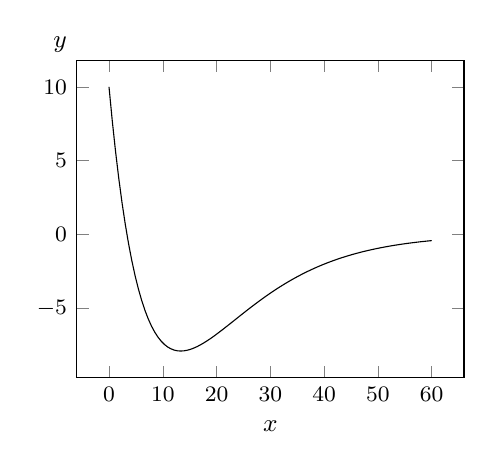
\begin{tikzpicture}
\begin{axis}[small,xlabel={$x$},ylabel={$y$},ylabel style={rotate=-90},ylabel style={at={(axis description cs:0,1.05)}}]
\addplot[domain=0:60,samples=100]{(10-3*x)*e^(-0.1*x)};
\end{axis}
\end{tikzpicture}
\caption{مثال \حوالہ{مثال_سادہ_دو_درجی_حقیقی_دوہرا_جذر} کا مخصوص حل۔}
\label{شکل_مثال_سادہ_دو_درجی_حقیقی_دوہرا_جذر}
\end{figure}
\انتہا{مثال}
%=============================

\حصہء{تیسری صورت: مخلوط جوڑی دار جذر}
امتیازی مساوات \حوالہ{مساوات_سادہ_دو_درجی_مستقل_عددی_سر_پ} میں \عددی{a^2-4c} کی قیمت منفی ہونے کی صورت میں مخلوط جوڑی دار
 جذر \عددی{\lambda=-\tfrac{a}{2}\mp i\omega} ملتے ہیں جہاں \عددی{\omega^2=b-\tfrac{a^2}{4}} کے برابر ہے۔ان سے مخلوط اساس لکھتے ہیں۔
\begin{align}\label{مساوات_سادہ_دو_درجی_مخلوط_اساس_الف}
y_{m1}=e^{(-\frac{a}{2}+i\omega)x},\quad y_{m2}=e^{(-\frac{a}{2}-i\omega)x}
\end{align}
اس مخلوط اساس سے حقیقی اساس حاصل کیا جائے گا۔ایسا کرنے کی خاطر ریاضی کے چند کلیات پر غور کرتے ہیں۔تفاعل \عددی{e^z}، جہاں \عددی{z=x+iy} مخلوط عدد ہے  جبکہ \عددی{x} اور \عددی{y} حقیقی اعداد ہیں، کو درج ذیل لکھا جا سکتا ہے۔
\begin{align*}
e^z=e^{x+iy}=e^xe^{iy}
\end{align*}
\عددی{e^{iy}} کی \اصطلاح{مکلارن تسلسل}\فرہنگ{مکلارن تسلسل}\فرہنگ{تسلسل!مکلارن}\حاشیہب{Maclaurin series}\فرہنگ{Maclaurin series} لکھ کر حقیقی اجزاء اور خیالی اجزاء کو علیحدہ علیحدہ قوسین میں اکٹھے کرتے ہیں۔یہاں \عددی{i^2=-1}، \عددی{i^3=-i}، \عددی{i^4=1} لئے گئے ہیں۔
\begin{align*}
e^{iy}&=1+\frac{iy}{1!}+\frac{(iy)^2}{2!}+\frac{(iy)^3}{3!}+\frac{(iy)^4}{4!}+\frac{(iy)^5}{5!}\cdots\\
&=\left(1-\frac{y^2}{2!}+\frac{y^4}{4!}-+\cdots\right) +i\left(\frac{y}{1!}-\frac{y^3}{3!}+\frac{y^5}{5!}-+\cdots\right)\\
&=\cos y+i\sin y
\end{align*}
آخری قدم پر آپ تسلی کر لیں کہ پہلی قوسین \عددی{\cos y} کی مکلارن تسلسل دیتی ہے جبکہ دوسری قوسین \عددی{\sin y} کی مکلارن تسلسل دیتی ہے۔ آپ اس کتاب میں آگے پڑھیں گے کہ درج بالا تسلسل میں اجزاء کی ترتیب بدلی جا سکتی ہے۔یوں ہم \اصطلاح{یولر مساوات}\فرہنگ{یولر مساوات}\حاشیہب{Euler equation}\فرہنگ{Euler equation}  
 \begin{align}\label{مساوات_سادہ_دو_درجی_یولر_مساوات_الف}
e^{iy}=\cos y+i\sin y
\end{align}
حاصل کرنے میں کامیاب ہوئے ہیں۔آپ دیکھ سکتے ہیں کہ
\begin{align}\label{مساوات_سادہ_دو_درجی_یولر_مساوات_ب}
e^{-iy}=\cos (-y)+i\sin (-y)=\cos y-i\sin y
\end{align}
مساوات \حوالہ{مساوات_سادہ_دو_درجی_یولر_مساوات_الف} اور مساوات \حوالہ{مساوات_سادہ_دو_درجی_یولر_مساوات_ب} کو جمع اور تفریق کرتے ہوئے درج ذیل کلیات حاصل ہوتے ہیں۔
\begin{align}
\cos y=\frac{e^{iy}+e^{-iy}}{2}, \quad \sin y=\frac{e^{iy}-e^{-iy}}{2i}
\end{align}
ہو گا۔یہ سب جاننے کے بعد آئیں مساوات \حوالہ{مساوات_سادہ_دو_درجی_مخلوط_اساس_الف} میں دیے مخلوط اساس پر دوبارہ غور کریں۔
\begin{align*}
y_{m1}&=e^{(-\frac{a}{2}+i\omega)x}=e^{-\frac{a}{2}x}e^{i\omega x}=e^{-\frac{a}{2}x} (\cos \omega x+i\sin \omega x)\\
y_{m2}&=e^{(-\frac{a}{2}-i\omega)x}=e^{-\frac{a}{2}x}e^{-i\omega x}=e^{-\frac{a}{2}x} (\cos \omega x-i\sin \omega x)
\end{align*}
چونکہ اساس کے اجزاء کو مستقل (حقیقی یا خیالی یا مخلوط) سے ضرب دے کر جمع کرتے ہوئے نیا حل حاصل کیا جا سکتا ہے لہٰذا ہم درج بالا دونوں اجزاء کو مستقل \عددی{\tfrac{1}{2}} سے ضرب دے کر جمع کرتے ہوئے ایک نیا اور حقیقی حل \عددی{y_1} دریافت کرتے ہیں۔
\begin{align*}
y_1=\frac{1}{2}y_{m1}+\frac{1}{2}y_{m2}=e^{-\frac{a}{2}x} \cos \omega x
\end{align*}
اسی طرح مخلوط اساس کے پہلے جزو  کو مستقل \عددی{\tfrac{1}{2i}} اور دوسرے جزو کو مستقل \عددی{-\tfrac{1}{2i}} سے ضرب دیتے ہوئے جمع کر کے نیا اور حقیقی حل \عددی{y_2} حاصل کرتے ہیں۔
\begin{align*}
y_2=\frac{1}{2i}y_{m1}-\frac{1}{2i}y_{m2}=e^{-\frac{a}{2}x} \sin \omega x
\end{align*}
درج بالا حاصل کردہ حقیقی تفاعل 
\begin{align}\label{مساوات_سادہ_دو_درجی_مخلوط_اساس_ب}
y_1=e^{-\frac{a}{2}x} \cos \omega x\quad y_2=e^{-\frac{a}{2}x} \sin \omega x
\end{align}
 کو از خود حل کا اساس تصور کیا جا سکتا ہے۔ یہاں غور کریں کہ ہم نے مخلوط جذر \عددی{\lambda=(-\tfrac{a}{2}\mp i \omega)x} سے حقیقی اساس  (مساوات \حوالہ{مساوات_سادہ_دو_درجی_مخلوط_اساس_ب}) حاصل کیا ہے۔ اس حقیقی اساس کو استعمال کرتے ہوئے عمومی حل لکھتے ہیں۔
\begin{align}
y=e^{-\frac{a}{2}x} (c_1 \cos \omega x+c_2 \sin \omega x)
\end{align}

 %==============================
%===============================
\ابتدا{مثال}\شناخت{مثال_سادہ_دو_درجی_مخلوط_جذر_الف}\quad مخلوط جذر، ابتدائی قیمت مسئلہ\\
درج ذیل ابتدائی قیمت مسئلے کو حل کریں۔
\begin{align*}
y''+0.36y'+9.0324y=0,\quad y(0)=0, \quad y'(0)=3
\end{align*}

حل:امتیازی مساوات \عددی{\lambda^2+0.36\lambda+9.0324=0} کے مخلوط جذر \عددی{\lambda=-0.18+\mp i3} ہیں لہٰذا عمومی حل
\begin{align*}
y=e^{-0.18x}(c_1 \cos 3x+c_2 \sin 3x)
\end{align*}
ہو گا۔مخصوص حل حاصل کرنے کی خاطر \عددی{c_1} اور \عددی{c_2} درکار ہیں جنہیں عمومی مساوات میں ابتدائی معلومات پر کرتے ہوئے حاصل کرتے ہیں۔پہلے ابتدائی معلومات سے
\begin{align*}
y(0)=e^{0}(c_1 \cos 0+c_2 \sin 0)=0, \quad c_1=0
\end{align*}
ملتا ہے۔عمومی حل کے تفرق
\begin{align*}
y'=-0.5e^{-0.5x}(c_1 \cos 3x+c_2 \sin 3x)+e^{-0.5x}(-3c_1 \sin 3x+3c_2 \cos 3x)
\end{align*}
میں دوسری ابتدائی معلومات پر کرتے ہوئے
\begin{align*}
y'=-0.5e^{0}(0 \cos 0+c_2 \sin 0)+e^{0}(0 \sin 0+3c_2 \cos 0)=3, \quad c_2=1
\end{align*}
ملتا ہے۔یوں مخصوص حل درج ذیل ہو گا۔
\begin{align*}
y=e^{-0.18x}\sin 3x
\end{align*}
شکل \حوالہ{شکل_مثال_سادہ_دو_درجی_مخلوط_جذر_الف} میں مخصوص حل دکھایا گیا ہے۔ساتھ ہی ساتھ، نقطہ دار لکیروں سے، سائن نما منحنی کے مثبت چوٹیوں کو چھوتا ہوا \اصطلاح{غلاف}\فرہنگ{غلاف}\حاشیہب{envelope}\فرہنگ{envelope} \عددی{e^{-0.18x}} اور منفی چوٹیوں کو چھوتا ہوا غلاف \عددی{-e^{-0.18x}} بھی دکھائے گئے ہیں۔مخصوص حل (\عددی{x} کو \عددی{t} لیتے ہوئے) \اصطلاح{قصری ارتعاش}\فرہنگ{قصری!ارتعاش}\فرہنگ{ارتعاش!قصری}\حاشیہب{damped oscillations}\فرہنگ{oscillations!damped} کو ظاہر کرتی ہے۔اگر \عددیء{y} فاصلے کو ظاہر کرتی ہو تب یہ میکانی قصری ارتعاش ہو گی اور اگر \عددی{y} برقی رو یا برقی دباو ہو تب یہ برقی قصری ارتعاش ہو گی۔
\begin{figure}
\centering
\begin{tikzpicture}
\begin{axis}[small,xlabel={$x$},ylabel={$y$},ylabel style={rotate=-90},ylabel style ={at={(axis description cs:0,1.05)}}]
\addplot[domain=0:25,samples=300] {e^(-0.18*x)*sin(3*x*180/pi)};
\addplot[dashed,domain=0:25]{e^(-0.18*x)}node[pos=0.15,pin=45:{غلاف}]{};
\addplot[dashed,domain=0:25]{-e^(-0.18*x)};
\end{axis}
\end{tikzpicture}
\caption{مثال \حوالہ{مثال_سادہ_دو_درجی_مخلوط_جذر_الف} کا مخصوص حل۔}
\label{شکل_مثال_سادہ_دو_درجی_مخلوط_جذر_الف}
\end{figure}

\انتہا{مثال}
%================================
\ابتدا{مثال}\quad مخلوط جذر\\
سادہ تفرقی مساوات
\begin{align*}
y''+\omega^2 y=0,\quad \text{\RL{($\omega$\, غیر صفر مستقل ہے)}}
\end{align*}
کا عمومی حل درج ذیل ہے۔
\begin{align*}
y=c_1 \cos \omega x+c_2 \sin \omega x
\end{align*}
\انتہا{مثال}
%================================

\begin{table}
\caption{تین صورتوں کی تفصیل}
\label{جدول_سادہ_دو_درجی_تین_صورتیں}
\centering
\begin{tabular}{rrrl}
صورت& مساوات \حوالہ{مساوات_سادہ_دو_درجی_مستقل_عددی_سر_پ} کے جذر & مساوات \حوالہ{مساوات_سادہ_دو_درجی_مستقل_عددی_سر_الف} کی اساس & مساوات \حوالہ{مساوات_سادہ_دو_درجی_مستقل_عددی_سر_الف} کا عمومی حل\\
\hline
پہلی & منفرد حقیقی \عددی{\lambda_1} ،\عددی{\lambda_2} & \عددی{e^{\lambda_1 x}}، \عددی{e^{\lambda_2 x}} & \عددی{y=c_1 e^{\lambda_1 x}+c_2 e^{\lambda_2 x}}  \\
دوسری& دوہرا جذر \عددی{\lambda=-\frac{a}{2}} & \عددی{e^{-\frac{a}{2}x}}، \عددی{xe^{-\frac{a}{2}x}} &  \عددی{y=(c_1+c_2 x)e^{-\frac{a}{2}x}}\\
تیسری& جوڑی دار مخلوط \عددی{\lambda=-\frac{a}{2} \mp i\omega} & \عددی{e^{-\frac{a}{2}x}\sin \omega x}،  \عددی{e^{-\frac{a}{2}x}\cos\omega x} & \عددی{y=e^{-\frac{a}{2}x}(c_1 \cos \omega x+c_2 \sin \omega x)}
\end{tabular}
\end{table}

جدول \حوالہ{جدول_سادہ_دو_درجی_تین_صورتیں} میں درج بالا تین صورتوں کی تفصیل اکٹھی کی گئی ہے۔یہ تین اقسام میکانی ارتعاش یا برقی ارتعاش کو ظاہر کرتی ہیں۔آپ تفرقی مساوات کی قوت یہاں سے جان سکتے ہیں۔آپس میں بالکل مختلف میدانوں (مثلاً میکانی اور برقی) کے مسائل ایک طرز  کی تفرقی مساوات سے ظاہر کئے جا سکتے ہیں۔ 
%====================================
%=====================================

\حصہء{سوالات}
سوال \حوالہ{سوال_سادہ_دو_درجی_مستقل-عددی_سر_الف} تا سوال \حوالہ{سوال_سادہ_دو_درجی_مستقل-عددی_سر_ب} کے عمومی حل حاصل کریں۔انہیں واپس تفرقی مساوات میں پر کرتے ہوئے ان کی درستگی ثابت کریں۔

%==================
\ابتدا{سوال}\شناخت{سوال_سادہ_دو_درجی_مستقل-عددی_سر_الف}
\begin{align*}
y''+4y=0
\end{align*}
جواب:\عددی{y=c_1\cos 2x+c_2 \sin 2x}
\انتہا{سوال}
%========================
\ابتدا{سوال}
\begin{align*}
4y''-9y=0
\end{align*}
جواب:\عددی{y=c_1e^{\frac{3}{2}x}+c_2 e^{-\frac{3}{2}x}}
\انتہا{سوال}
%========================
\ابتدا{سوال}
\begin{align*}
y''+5y'+6y=0
\end{align*}
جواب:\عددی{y=c_1e^{-2x}+c_2e^{-3x}}
\انتہا{سوال}
%========================
\ابتدا{سوال}
\begin{align*}
y''+2\pi y'+\pi^2 y=0
\end{align*}
جواب:\عددی{y=(c_1+c_2 x)e^{-\pi x}}
\انتہا{سوال}
%========================
\ابتدا{سوال}
\begin{align*}
y''-6 y'+9 y=0
\end{align*}
جواب:\عددی{y=(c_1+c_2 x)e^{3x}}
\انتہا{سوال}
%========================
\ابتدا{سوال}
\begin{align*}
4y''-12 y'+9 y=0
\end{align*}
جواب:\عددی{y=(c_1+c_2 x)e^{\tfrac{3}{2}x}}
\انتہا{سوال}
%========================
\ابتدا{سوال}
\begin{align*}
4y''+4 y'-3 y=0
\end{align*}
جواب:\عددی{y=c_1e^{\tfrac{x}{2}}+c_2 e^{-\tfrac{3}{2}x}}
\انتہا{سوال}
%========================
\ابتدا{سوال}
\begin{align*}
y''-5 y'+6 y=0
\end{align*}
جواب:\عددی{y=c_1e^{3x}+c_2e^{2x}}
\انتہا{سوال}
%========================
\ابتدا{سوال}\شناخت{سوال_سادہ_دو_درجی_مستقل-عددی_سر_ب}
\begin{align*}
9y''-30 y'+25 y=0
\end{align*}
جواب:\عددی{y=(c_1+c_2 x)e^{\tfrac{5}{3}x}}
\انتہا{سوال}
%========================

سوال \حوالہ{سوال_سادہ_دو_درجی_مستقل-عددی_سر_پ} تا سوال \حوالہ{سوال_سادہ_دو_درجی_مستقل-عددی_سر_ت} میں اساس سے تفرقی مساوات \عددی{y''+ay'+by=0} حاصل کریں۔

%======================
\ابتدا{سوال}\شناخت{سوال_سادہ_دو_درجی_مستقل-عددی_سر_پ}
\begin{align*}
e^{0.2x}, \quad e^{-0.5x}
\end{align*}
جواب:\عددی{y''+0.3y'-0.1y=0}
\انتہا{سوال}
%=======================
\ابتدا{سوال}
\begin{align*}
e^{-0.66x}, \quad e^{-0.32x}
\end{align*}
جواب:\عددی{y''+0.98y'+0.2112y=0}
\انتہا{سوال}
%=======================
\ابتدا{سوال}
\begin{align*}
\cos (4\pi x), \quad \sin (4\pi x)
\end{align*}
جواب:\عددی{y''+16\pi^2 y=0}
\انتہا{سوال}
%=======================
\ابتدا{سوال}
\begin{align*}
e^{(-2+i3)x}, \quad e^{(-2-i3)x}
\end{align*}
جواب:\عددی{y''+4y''+13y=0}
\انتہا{سوال}
%=======================
\ابتدا{سوال}\شناخت{سوال_سادہ_دو_درجی_مستقل-عددی_سر_ت}
\begin{align*}
e^{-1.7x}\cos 6.2 x, \quad e^{-1.7x}\sin 6.2x
\end{align*}
جواب:\عددی{y''+3.4y''+41.33y=0}
\انتہا{سوال}
%=======================

سوال \حوالہ{سوال_سادہ_دو_درجی_مستقل-عددی_سر_ٹ} تا سوال \حوالہ{سوال_سادہ_دو_درجی_مستقل-عددی_سر_ث} ابتدائی قیمت سوالات ہیں۔ان کے مخصوص حل دریافت کریں۔

%================
\ابتدا{سوال}\شناخت{سوال_سادہ_دو_درجی_مستقل-عددی_سر_ٹ}
\begin{align*}
y''+2y=0,\quad y(0)=5,\quad y'(0)=2
\end{align*}
جواب:\عددی{y=5\cos \sqrt{2} x+\sqrt{2}\sin \sqrt{2} x}
\انتہا{سوال}
%===========================
\ابتدا{سوال}
\begin{align*}
y''-25y=0,\quad y(0)=2,\quad y'(0)=-3
\end{align*}
جواب:\عددی{y=0.7e^{5x}+1.3e^{-5x}}
\انتہا{سوال}
%===========================
\ابتدا{سوال}
\begin{align*}
y''-y''-6y=0,\quad y(0)=0,\quad y'(0)=1
\end{align*}
جواب:\عددی{y=\tfrac{1}{5}(e^{3x}-e^{-2x})}
\انتہا{سوال}
%===========================
\ابتدا{سوال}
\begin{align*}
4y''+4y''+37y=0,\quad y(0)=0,\quad y'(0)=3
\end{align*}
جواب:\عددی{y=e^{-\tfrac{x}{2}}\sin 3x}
\انتہا{سوال}
%===========================
\ابتدا{سوال}
\begin{align*}
9y''+12y''+49y=0,\quad y(0)=2,\quad y'(0)=-1
\end{align*}
جواب:\عددی{y=e^{-\tfrac{2}{3}x}(2\cos \sqrt{5}x+\tfrac{1}{3\sqrt{5}}\sin \sqrt{5}x)}
\انتہا{سوال}
%===========================
\ابتدا{سوال}
\begin{align*}
y''-6y''+25y=0,\quad y(0)=0,\quad y'(0)=0.1
\end{align*}
جواب:\عددی{y=\tfrac{1}{40}e^{3x}\sin 4x}
\انتہا{سوال}
%===========================
\ابتدا{سوال}
\begin{align*}
y''+y=0,\quad y(0)=1,\quad y'(0)=1
\end{align*}
جواب:\عددی{y=\cos x+\sin x}
\انتہا{سوال}
%===========================
\ابتدا{سوال}\شناخت{سوال_سادہ_دو_درجی_مستقل-عددی_سر_ث}
\begin{align*}
8y''-2y'-y=0,\quad y(0)=2.2,\quad y'(0)=3.4
\end{align*}
جواب:\عددی{y=\tfrac{79}{15}e^{\tfrac{x}{2}}-\tfrac{46}{15}e^{-\tfrac{x}{4}}}
\انتہا{سوال}
%===========================

عمومی حل کے حصول میں خطی طور غیر تابع تفاعل نہایت اہم ہیں۔صرف ایسے تفاعل سے اساس حاصل ہوتا ہے۔دیے وقفے پر سوال \حوالہ{سوال_سادہ_دو_درجی_مستقل-عددی_سر_ج} تا سوال \حوالہ{سوال_سادہ_دو_درجی_مستقل-عددی_سر_چ} میں دیے تفاعل میں خطی طور تابع اور غیر تابع کی نشاندہی کریں۔ 
%================

\ابتدا{سوال}\شناخت{سوال_سادہ_دو_درجی_مستقل-عددی_سر_ج}
\begin{align*}
\cos kx, \quad \sin kx, \quad -\infty <x<\infty
\end{align*}
جواب:چونکہ \عددی{\tfrac{\sin kx}{\cos kx}} کی قیمت \عددی{x} تبدیل کرنے سے تبدیل ہوتی ہے لہٰذا یہ تفاعل خطی طور غیر تابع ہیں۔
\انتہا{سوال}
%============================
\ابتدا{سوال}
\begin{align*}
e^{kx}, \quad e^{-kx}\quad -\infty <x<\infty
\end{align*}
جواب:خطی طور غیر تابع
\انتہا{سوال}
%============================
\ابتدا{سوال}
\begin{align*}
x, \quad x^2\quad x>1
\end{align*}
جواب:خطی طور غیر تابع
\انتہا{سوال}
%============================
\ابتدا{سوال}
\begin{align*}
x\ln x, \quad x^2 \ln x\quad x>1
\end{align*}
جواب:خطی طور غیر تابع
\انتہا{سوال}
%============================

\ابتدا{سوال}\شناخت{سوال_سادہ_دو_درجی_مستقل-عددی_سر_چ}
\begin{align*}
x\ln x, \quad x\ln x^2 \ln x\quad x>1
\end{align*}
جواب:خطی طور تابع
\انتہا{سوال}
%============================
\ابتدا{سوال}\شناخت{سوال_سادہ_دو_درجی_غیر_مستحکم_الف}\quad غیر مستحکم صورت حال\\
ابتدائی قیمت مسئلہ \عددی{y''-4y=0} میں ابتدائی قیمتیں \عددی{y(0)=1} اور \عددی{y'(0)=-2} لیتے ہوئے مخصوص حل حاصل کریں۔مخصوص حل کو دوبارہ ابتدائی معلومات \عددی{y(0)=1.001} اور \عددی{y'(0)=-1.998} کے لئے حاصل کریں۔


\begin{figure}
\centering
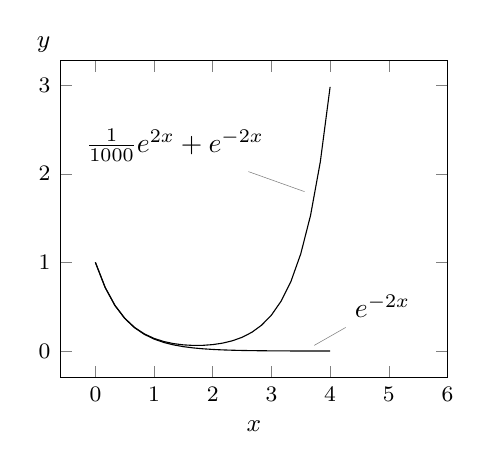
\begin{tikzpicture}
\begin{axis}[small,xmax=6,xlabel={$x$},ylabel={$y$},ylabel style={rotate=-90},ylabel style={at={(axis description cs:0,1.05)}}]
\addplot[domain=0:4]{e^(-2*x)}node[pos=0.9,pin=30:{$e^{-2x}$}]{};
\addplot[domain=0:4]{1/1000*e^(2*x)+e^(-2*x)}node[pos=0.8,pin=150:{$\frac{1}{1000}e^{2x}+e^{-2x}$}]{};
\end{axis}
\end{tikzpicture}
\caption{سوال \حوالہ{سوال_سادہ_دو_درجی_غیر_مستحکم_الف} کے منحنی حل۔}
\label{شکل_سوال_سادہ_دو_درجی_غیر_مستحکم_الف}
\end{figure}

جوابات:\عددی{y=e^{-2x}} اور \عددی{y=\tfrac{1}{1000}e^{2x}+e^{-2x}}؛ شکل \حوالہ{شکل_سوال_سادہ_دو_درجی_غیر_مستحکم_الف} میں دونوں حل دکھائے گئے ہیں۔آپ دیکھ سکتے ہیں کہ ابتدائی قیمتوں میں انتہائی کم فرق حل پر بہت زیادہ اثر ڈالتی ہیں۔یہ \اصطلاح{غیر مستحکم}\فرہنگ{غیر مستحکم!صورت}\حاشیہب{instability}\فرہنگ{instability}  صورت کو ظاہر کرتی ہے۔زلزلے\فرہنگ{زلزلہ}  میں غیر مستحکم عمارتیں\فرہنگ{عمارت} انہیں وجوہات پر ڈھیر ہوتی ہیں۔فضا میں ہوا کا دباو، درجہ حرارت اور نمی کی تناسب بھی غیر مستحکم صورت پیدا کرتے ہوئے  تباہ کن آندھیوں کا سبب بنتی ہیں۔
\انتہا{سوال}
%=========================
\ابتدا{سوال}
استمراری مساوات کے جذر \عددی{\lambda_1=-2} اور \عددی{\lambda_2=3} ہیں۔مساوات \حوالہ{مساوات_سادہ_دو_درجی_مستقل_عددی_سر_الف} حاصل کریں۔

جواب:\عددی{y''-y'-6y=0} 
\انتہا{سوال}
%========================
\ابتدا{سوال}
استمراری مساوات کے جذر \عددی{\lambda_1} اور \عددی{\lambda_2} ہیں۔مساوات \حوالہ{مساوات_سادہ_دو_درجی_مستقل_عددی_سر_الف} میں  \عددی{a} اور \عددی{b} حاصل کریں۔ یوں جذر جانتے ہوئے تفرقی مساوات حاصل کی جا سکتی ہے۔

جواب:\عددی{a=-\lambda_1-\lambda_2}، \عددی{b=\lambda_1 \lambda_2}
\انتہا{سوال}
%========================
\ابتدا{سوال}
تفرقی مساوات \عددی{y''+ky'=0} کو موجودہ طریقے سے حل کریں۔ اسی کو تخفیف درجہ کی ترکیب سے بھی حل  کریں۔دونوں جواب کیوں یکساں ہونا ضروری ہے۔

جواب:\عددی{y=c_1+c_2e^{-kx}}؛ یکتائیت۔ 
\انتہا{سوال}
%=======================
\ابتدا{سوال}
دوہرا جذر کو منفرد \عددی{\lambda_1} اور \عددی{\lambda_2} کی وہ صورت تصور کی جا سکتی ہے جب \عددی{\lambda_2 \to \lambda_1} ہو۔\عددی{\lambda_2=\lambda_1+\Delta \lambda} لیتے اور ایک حل \عددی{=e^{\lambda_1 x}} لیتے ہوئے اساس کا دوسرا رکن  \عددی{xe^{\lambda_1 x}} تلاش کریں۔

حل:دوسرا حل \عددی{e^{\lambda_2 x}=e^{(\lambda_1 +\Delta \lambda)x}=e^{\lambda_1 x}e^{\Delta \lambda x}} ہے۔\عددی{e^{\Delta \lambda x}} کا مکلارن تسلسل لیتے ہوئے \عددی{\Delta \lambda \to 0} کی بنا صرف پہلے دو ارکان لیتے ہیں۔
یوں  \عددی{e^{\Delta \lambda x}=1+\frac{\Delta \lambda x}{1!}+\frac{(\Delta \lambda x)^2}{2!}+\cdots \approx 1+\Delta \lambda x} ہو گا اور 
\عددی{e^{\lambda_2 x}=e^{\lambda_1 x}+\Delta \lambda xe^{\lambda_1 x}} لکھا جا سکتا ہے۔اب چونکہ \عددی{e^{\lambda_1 x}} پہلے سے اساس کا حصہ ہے لہٰذا اساس کا دوسرا رکن \عددی{xe^{\lambda_1 x}} ہو گا جہاں \عددی{\Delta \lambda} کو مستقل تصور کرتے ہوئے رد کیا جاتا ہے
\انتہا{سوال}

\حصہ{تفرقی عامل}
آپ \عددی{y=\sin x} یا \عددی{y=\tfrac{\dif f(x)}{\dif x}} کے عمل سے بخوبی واقف ہیں۔پہلی مثال میں کسی مقدار یا تفاعل \عددی{x} پر عامل \عددی{\sin} عمل کرتے ہوئے ایک نیا تفاعل دیتا ہے۔یوں \عددی{x=\tfrac{\pi}{2}} پر \عددی{\sin \tfrac{\pi}{2}=1} حاصل ہوتا ہے۔ ہم کہتے ہیں کہ \اصطلاح{عامل}\فرہنگ{عامل}\حاشیہب{operator}\فرہنگ{operator} \عددی{\sin} تفاعل \عددی{x} کے نقطہ \عددی{x=\tfrac{\pi}{2}} سے مبدل تفاعل \عددی{y} کا نقطہ \عددی{y=1} دیتا ہے۔اسی طرح \اصطلاح{عامل} \عددی{\tfrac{\dif}{\dif x}} تفاعل \عددی{x^3} پر عمل کرتے ہوئے تفاعل \عددی{3x^2} دیتا ہے۔

یہ بتلاتا چلوں کہ ریاضیات اور طبیعیات میں عامل کا استعمال نہایت اہم کردار ادا کرتا ہے۔ یہاں بالخصوص \اصطلاح{کوانٹم میکانیات}\فرہنگ{کوانٹم میکانیات}\حاشیہب{quantum mechanics}\فرہنگ{quantum mechanics} کا ذکر کرنا لازم جہاں عامل کا استعمال کثرت سے کیا جاتا ہے۔ 

اس کتاب میں ہم صرف \اصطلاح{تفرقی عامل}\فرہنگ{تفرقی!عامل}\فرہنگ{عامل!تفرقی}\حاشیہب{differential operator}\فرہنگ{operator!differential}\فرہنگ{differential!operator} \عددی{D} پر بحث کریں گے جہاں \عددی{D=\tfrac{\dif}{\dif x}} ہے۔ یوں ایک درجی تفرق
\begin{align}
Dy=y'=\frac{\dif y}{\dif x}
\end{align}
لکھا جائے گا۔اسی طرح دو درجی تفرق \عددی{D^2y=D(Dy)=y''} اور تین درجی تفرق \عددی{D^3 y=y'''} لکھا جائے گا۔اس طرح \عددی{D \sin x=\cos x} اور \عددی{D^2 \sin x=-\sin x} ہو گا۔

خطی متجانس مساوات \عددی{y''+ay'+by=0} جہاں \عددی{a} اور \عددی{b} مستقل مقدار ہیں میں \اصطلاح{دو درجی تفرقی عامل}
\begin{align*}
L=P(D)=D^2+aD+bI
\end{align*}
متعارف کرتے ہیں جہاں \عددی{I} \اصطلاح{مماثلی عامل}\فرہنگ{عامل!مماثلی}\فرہنگ{مماثلی!عامل}\حاشیہب{identity operator}\فرہنگ{operator!identity}\فرہنگ{identity!operator} ہے جس کی تعریف \عددی{Iy=y} ہے۔اس طرح دیے گئے تفرقی مساوات کو درج ذیل لکھا جا سکتا ہے۔
\begin{align}\label{مساوات_سادہ_دو_درجی_کثیر_رکنی_تفرقی_عامل_الف}
Ly=P(D)y=(D^2+aD+bI)y=0
\end{align}
\عددی{L} خطی عامل اور \عددی{P} کثیر رکنی\فرہنگ{کثیر رکنی}\حاشیہب{polynomial}\فرہنگ{polynomial} ہے۔یوں اگر \عددی{Lw} اور \عددی{Ly} پائے جاتے ہوں (یعنی \عددی{w} اور \عددی{y} دو مرتبہ قابل تفرق ہوں) تب \عددی{L(cy+kw)} بھی پایا جاتا ہے جہاں \عددی{c} اور \عددی{k} کوئی مستقل ہیں۔مزید درج ذیل لکھا جا سکتا ہے۔
\begin{align}
L(cy+kw)=cLy+kLw
\end{align}

چونکہ \عددی{De^{\lambda x}=\lambda e^{\lambda x}} اور \عددی{D^2 e^{\lambda x}=\lambda^2 e^{\lambda x}} ہیں لہٰذا 
\begin{gather}
\begin{aligned}
Le^{\lambda x}&=(D^2+aD+bI)e^{\lambda x}\\
&=(\lambda^2+a\lambda+b)e^{\lambda x}=P(\lambda) e^{\lambda x}=0
\end{aligned}
\end{gather}
ہو گا۔حصہ \حوالہ{حصہ_سادہ_دو_درجی_مستقل_عددی_سر} میں بھی ہم نے یہی نتیجہ اخذ کیا تھا کہ \عددی{e^{\lambda x}} صرف اور صرف اس صورت اس تفرقی مساوات کا حل ہو گا اگر \عددی{\lambda} امتیازی مساوات \عددی{P(\lambda)=0} کا جذر ہو۔

یہاں دلچسپ بات یہ ہے کہ \عددی{P(\lambda)} عام الجبرائی کثیر رکنی ہے جس کی تجزی\فرہنگ{تجزی}\حاشیہب{factorization}\فرہنگ{factorization} کی جا سکتی ہے۔\عددی{\lambda} کی جگہ \عددی{D} پر کرنے سے  \اصطلاح{کثیر رکنی عامل} حاصل ہوتا ہے۔
%================================

\ابتدا{مثال}\quad تفرقی مساوات کا حل بذریعہ تجزی\\
کثیر رکنی \عددی{P(D)=D^2+4D-21I} کی تجزی سے \عددی{P(D)=0} کو حل کریں۔

حل:\عددی{I^2=1} لیتے ہوئے \عددی{D^2+4D-21I=(D-3)(D+7)} لکھا جا سکتا ہے۔اب \عددی{(D-3)y=y'-3y=0} کا حل \عددی{y_1=e^{3x}} اور \عددی{()y=y'+7y=0} کا حل \عددی{y_2=e^{-7x}} ہے۔یہ جوابات کسی بھی وقفے پر حل کی اساس ہیں۔آئیں تفرقی مساوات حاصل کریں۔
\begin{align*}
(D-3)(D+7)y=(D-3)(y'+7y)=y''+7y'-3y'-21y=y''+4y'-21y=0
\end{align*}
\انتہا{مثال}
%===============================

مساوات \حوالہ{مساوات_سادہ_دو_درجی_کثیر_رکنی_تفرقی_عامل_الف} میں کثیر رکنی کے عددی سر مستقل مقدار ہیں۔ایسی صورت میں تفرقی عامل کے استعمال سے تفرقی مساوات حل کرنا نہایت آسان ثابت ہوتا ہے۔عددی سر مستقل نہ ہونے کی صورت میں تفرقی عامل کا استعمال نہایت پیچیدہ ثابت ہوتا ہے جس پر اس کتاب میں تبصرہ نہیں کیا جائے گا۔

%===================================
%===================================

\حصہء{سوالات}
سوال \حوالہ{سوال_سادہ_دو_درجی_تفرقی_عامل_الف} تا سوال \حوالہ{سوال_سادہ_دو_درجی_تفرقی_عامل_ب} دیے تفاعل پر دیا تفرقی عامل لاگو کریں۔
  
%===============
\ابتدا{سوال}\شناخت{سوال_سادہ_دو_درجی_تفرقی_عامل_الف}
\begin{align*}
D+2I; \quad x^3, \quad \cos 5x, \quad e^{-kx}, \quad \cosh x
\end{align*}
جوابات:\عددی{3x^2+2x^3}، \عددی{-5\sin 5x+2\cos 5x}، \عددی{(2-k)e^{-kx}}، \عددی{\sinh x+2\cosh x}
\انتہا{سوال}
%=======================
\ابتدا{سوال}
\begin{align*}
D^2-3D; \quad 2x^4-x, \quad 2\sinh 2x-\cos 5x
\end{align*}
جوابات:\عددی{24x^2-24x^3+3}، \عددی{-15\sin 5x-12\cosh 2x+25\cos 5x+\sinh 2x}
\انتہا{سوال}
%==================================
\ابتدا{سوال}
\begin{align*}
(D+2I)^2; \quad e^{3x}, \quad xe^{2x}
\end{align*}
جوابات:\عددی{25e^{3x}}، \عددی{(12x+8)e^{2x}}
\انتہا{سوال}
%==================================
\ابتدا{سوال}
\begin{align*}
(D-3I)^2; \quad e^{2x}, \quad xe^{3x}
\end{align*}
جوابات:\عددی{e^{2x}}، \عددی{0}
\انتہا{سوال}
%==================================
\ابتدا{سوال}\شناخت{سوال_سادہ_دو_درجی_تفرقی_عامل_ب}
\begin{align*}
(D+I)(D-2I); \quad e^{2x}, \quad xe^{2x}
\end{align*}
جوابات:\عددی{-2e^{2x}}، \عددی{2(1-x)e^{2x}}
\انتہا{سوال}
%==================================

سوال \حوالہ{سوال_سادہ_دو_درجی_تفرقی_عامل_پ} تا سوال \حوالہ{سوال_سادہ_دو_درجی_تفرقی_عامل_ت} کی تجزی حاصل کرتے ہوئے حل کریں۔

%==============================
\ابتدا{سوال}\شناخت{سوال_سادہ_دو_درجی_تفرقی_عامل_پ}
\begin{align*}
(D^2-9I)y=0
\end{align*}
جواب:\عددی{y=c_1e^{3x}+c_2e^{-3x}}
\انتہا{سوال}
%===========================
\ابتدا{سوال}
\begin{align*}
(D^2+4D+4I)y=0
\end{align*}
جواب:دوہرا جذر پایا جاتا ہے لہٰذا دوسرا حل \عددی{xe^{2x}} لیتے ہوئے \عددی{y=(c_1+c_2 x)e^{2x}} ملتا ہے۔
\انتہا{سوال}
%===========================
\ابتدا{سوال}
\begin{align*}
(D^2+4D+13I)y=0
\end{align*}
جواب:\عددی{y=e^{-2x}(c_1 \cos 3x+c_2 \sin 3x)}
\انتہا{سوال}
%===========================
\ابتدا{سوال}
\begin{align*}
(4D^2+4D-17I)y=0
\end{align*}
جواب:\عددی{y=e^{\tfrac{x}{2}}(c_1 \cos 2x+c_2 \sin 2x)}
\انتہا{سوال}
%===========================
\ابتدا{سوال}\شناخت{سوال_سادہ_دو_درجی_تفرقی_عامل_ت}
\begin{align*}
(9D^2+12D+4I)y=0
\end{align*}
جواب:دوہرا جذر پایا جاتا ہے۔ \عددی{y=(c_1+c_2 x)e^{-\tfrac{2}{3}x}}
\انتہا{سوال}
%===========================
%===========================

\حصہ{اسپرنگ سے جڑی کمیت کی آزادانہ ارتعاش}
مستقل قیمت کے عددی سر والے خطی سادہ تفرقی مساوات  میکانی ارتعاش میں کلیدی کردار ادا کرتے ہیں۔اس حصے میں اسپرنگ سے جڑی کمیت کی حرکت پر غور کیا جائے گا۔اس نظام کو \اصطلاح{اسپرنگ اور کمیت}\فرہنگ{اسپرنگ!کمیت}\فرہنگ{کمیت!اسپرنگ}\فرہنگ{ارتعاش!اسپرنگ اور کمیت} کا نظام کہا جائے گا جسے شکل \حوالہ{شکل_سادہ_دو_درجی_اسپرنگ_کمیت_نظام} میں دکھایا گیا ہے۔
\begin{figure}
\centering
\begin{tikzpicture}
\node[circle,fill=gray,inner sep=2.5mm] (a) at (0,0) {};
\node[circle,fill=gray,inner sep=2.5mm] (b) at (3,2) {};
\node[circle,inner sep=2.5mm] (c) at (6,2.5) {};
\draw[decoration={aspect=0.3, segment length=3mm, amplitude=3mm,coil},decorate] (0,5) -- (a); 
\draw[decoration={aspect=0.3, segment length=1.7mm, amplitude=3mm,coil},decorate] (3,5) -- (b); 
\draw[decoration={aspect=0.3, segment length=1.5mm, amplitude=3mm,coil},decorate] (6,5) -- (c); 
\fill [pattern = north east lines] (-1,5) rectangle (7,5.2);
\draw[thick] (-1,5) -- (7,5);
%dashed lines
\draw  (c)++(0,0.37) node[below]{\RL{ڈھیلا اسپرنگ}};
\draw[dashed] (c)++(0.5,0.37)coordinate(cR)--++(-2.75,0)coordinate(cL);
\draw  (b)++(0,-0.37) node[below]{\RL{ساکن نظام}};
\draw[dashed] (b)++(1.5,0.37)coordinate(bR)--++(-3.75,0)coordinate(bL);
\draw  (a)++(0,-0.37) node[below]{\RL{ارتعاش پذیر نظام}};
\draw[dashed] (a)++(0,0.37)coordinate(aR)--++(2.3,0)coordinate(aL);
%dimensions
\draw[stealth-stealth] (cL)++(0.5,0)coordinate(cT)--($(bL)!(cT)!(bR)$)node[pos=0.5, right]{$s_0$};
\draw[-stealth] (bL)++(0.2,0)coordinate(bT)--($(aL)!(bT)!(aR)$)node[pos=0.5, right]{$y$};
\draw(b)++(-0.5,0.37)node[left,fill=white]{$(y=0)$};
\end{tikzpicture}
\caption{اسپرنگ اور کمیت کا نظام۔}
\label{شکل_سادہ_دو_درجی_اسپرنگ_کمیت_نظام}
\end{figure}

ایک عام اسپرنگ جو لمبائی میں اضافہ اور کمی کو روکتا ہو کو شکل \حوالہ{شکل_سادہ_دو_درجی_اسپرنگ_کمیت_نظام} میں مستحکم سلاخ سے لٹکایا ہوا دکھایا گیا ہے۔اس کی نچلی سر سے کمیت \عددی{m} کی لوہے کا گیند لٹکانے سے  اسپرنگ کی لمبائی میں  \عددی{s_0} اضافہ پیدا ہوتا ہے۔اس ساکن نظام میں اسپرنگ کے نچلے سر کو \عددی{y=0} تصور کیا جاتا ہے۔ہم نیچے رخ کو مثبت رخ تصور کرتے ہیں۔یوں نیچے رخ  قوت کو مثبت اور اوپر رخ  قوت کو منفی تصور کیا جائے گا۔اسی طرح مقام \عددی{y=0} سے نیچے رخ  فاصلہ \عددی{y} مثبت ہو گا۔مزید اسپرنگ کی کمیت کو گیند کی کمیت سے اتنا کم تصور کیا جاتا ہے کہ اسپرنگ کی کمیت کو درج ذیل تبصرے میں رد کیا جا سکتا ہے۔

ساکن حالت میں اسپرنگ پر نیچے رخ قوت \عددی{mg} عمل کرتا ہے جس سے  اسپرنگ  کی لمبائی میں \عددی{s_0} اضافہ پیدا ہوتا ہے۔ یہاں \عددی{g=\SI{9.8}{\meter\per\second\squared}} ثقلی اسراع اور \عددی{mg} گیند کا وزن ہے۔اسپرنگ کی لمبائی میں اضافے  کی وجہ سے، \اصطلاح{قانون ہک}\فرہنگ{قانون ہک}\فرہنگ{ہک کا قانون}\حاشیہب{Hooke's law}\فرہنگ{Hooke's law} کے تحت\حاشیہد{روبرٹ ہک (1635-1703) انگلستان  کے ماہر طبیعیات تھے۔}، اسپرنگ اوپر رخ  \اصطلاح{بحالی قوت}\فرہنگ{بحالی قوت}\فرہنگ{قوت!بحالی}\حاشیہب{restoring force}\فرہنگ{restoring force}\فرہنگ{force!restoring}  \عددی{F_0=-ks_0} پیدا کرتا ہے جہاں \عددی{k} \اصطلاح{اسپرنگ مستقلہ}\فرہنگ{اسپرنگ!مستقلہ}\فرہنگ{مستقل!اسپرنگ}\حاشیہب{spring constant}\فرہنگ{spring constant} ہے۔بحالی قوت اسپرنگ کی لمبائی میں تبدیلی کو روکنے کی کوشش کرتا ہے۔قوت \عددی{mg} مثبت رخ ہے لہٰذا اس کو مثبت لکھا گیا ہے جبکہ قوت \عددی{-k s_0} منفی رخ ہے لہٰذا اس کو منفی لکھا گیا ہے۔ان قوتوں کا مجموعہ صفر \عددی{mg-ks_0=0} کے برابر ہوتا ہے۔اگر ان قوتوں کا مجموعہ صفر کے برابر نہ ہوتا تو گیند ساکن نہ ہوتا بلکہ نیوٹن کے قانون \عددی{ّF=my''} کے تحت حرکت کرتا۔طاقتور اسپرنگ کے مستقلہ \عددی{k} کی قیمت زیادہ ہوتی ہے۔ان دونوں قوتوں کی مقدار گیند کی حرکت سے تبدیل نہیں ہوتی لہٰذا ان کا مجموعہ ہر وقت صفر کے برابر ہو گا۔یوں گیند کی حرکت میں ان دونوں قوتوں کا کوئی کردار نہیں ہے لہٰذا ان پر مزید بات نہیں کی جائے گی۔

فرض کریں کہ گیند کو نیچے رخ کھینچ کر چھوڑا جاتا ہے۔شکل \حوالہ{شکل_سادہ_دو_درجی_اسپرنگ_کمیت_نظام} میں گیند کو ساکن مقام سے لمحاتی طور \عددی{y} فاصلے پر دکھایا گیا ہے۔اس لمحہ اسپرنگ اضافی بحالی قوت \عددی{F_1=-ky} پیدا کرتا ہے جس کے تحت گیند نیوٹن کے قانون
\begin{align}
F_1=ma = my''
\end{align}
 کے تحت حرکت کرے گا جہاں \عددی{y''=\tfrac{\dif^2 y}{\dif t^2}} ہے۔

\حصہء{بلا تقصیر حرکت کی سادہ تفرقی مساوات}
ہر نظام تقصیری ہوتا ہے ورنہ حرکت کبھی بھی نہ رکتی۔ نہایت کم تقصیری نظام  جس کے حرکت کا مطالعہ نسبتاً کم دورانیے کے لئے  کیا جائے میں تقصیر کو نظر انداز کیا جا سکتا ہے۔یوں اس کو غیر تقصیری تصور کیا جا سکتا ہے۔ شکل \حوالہ{شکل_سادہ_دو_درجی_اسپرنگ_کمیت_نظام} کا نظام غیر تقصیری نظام کی عمدہ مثال ہے۔نیوٹن کے قانون کو بروئے کار لیتے ہوئے اس نظام کی تفرقی مساوات لکھتے ہیں۔
\begin{align}
my''+ky=0
\end{align}
یہ مستقل عددی سر والا خطی متجانس سادہ تفرقی مساوات ہے جس کا امتیازی مساوات \عددی{\lambda^2+\tfrac{k}{m}=0} ہے۔امتیازی مساوات کے جوڑی دار مخلوط جذر \عددی{\lambda=\mp i \sqrt{\tfrac{k}{m}}=\mp i \omega_0} ہیں جن سے عمومی حل لکھتے ہیں۔
\begin{align}\label{مساوات_سادہ_دو_درجی_اسپرنگ_کمیت_ارتعاش_الف}
y=A \cos \omega_0 t+B \sin \omega_0 t \quad \quad \omega_0=\sqrt{\frac{k}{m}}
\end{align}
اس حرکت کو \اصطلاح{ہارمونی ارتعاش}\فرہنگ{ہارمونی ارتعاش}\حاشیہب{harmonic oscillation}\فرہنگ{harmonic oscillation} کہتے ہیں جس کی \اصطلاح{تعدد}\فرہنگ{تعدد}\حاشیہب{frequency}\فرہنگ{frequency}  \عددی{f_0=\frac{\omega_0}{2\pi}} \اصطلاح{ہرٹز}\فرہنگ{ہرٹز}\حاشیہب{Hertz}\فرہنگ{Hertz} ہے\حاشیہد{ہائنرک ہرٹز (1857-1894) جرمنی کے ماہر طبیعیات تھے جنہوں نے برقناطیسی امواج دریافت کئے۔}۔تعدد \عددی{f_0} کو نظام کی \اصطلاح{قدرتی تعدد}\فرہنگ{قدرتی تعدد}\فرہنگ{تعدد!قدرتی}\حاشیہب{natural frequency}\فرہنگ{natural frequency} کہتے ہیں۔

\عددی{C=\sqrt{A^2+B^2}} اور \عددی{\delta=\tan^{-1} \tfrac{B}{A}} لیتے ہوئے مساوات \حوالہ{مساوات_سادہ_دو_درجی_اسپرنگ_کمیت_ارتعاش_الف} کو 
\begin{align}\label{مساوات_سادہ_دو_درجی_اسپرنگ_کمیت_ارتعاش_ب}
y=C\cos(\omega_0 t-\delta)
\end{align}
لکھا جا سکتا ہے جہاں \عددی{C} \اصطلاح{حیطہ}\فرہنگ{حیطہ}\حاشیہب{amplitude}\فرہنگ{amplitude} اور \عددی{\delta} \اصطلاح{زاویائی فرق}\فرہنگ{زاویائی فرق}\حاشیہب{phase angle}\فرہنگ{phase angle} کہلاتے ہیں۔  
\begin{figure}
\centering
\begin{tikzpicture}
\begin{axis}[small,axis lines*=middle,xlabel={$t$},ylabel={$y$},ylabel style={rotate=-90},xtick=\empty,ytick=\empty,xmin=0,ylabel style={at={(axis description cs:0,1.05)}},xlabel style={at={(axis description cs:1.05,0.475)}}]
\addplot[domain=0:360,samples=100]{cos(x)}node[pos=0.2,fill=white]{ب};
\addplot[domain=0:360,samples=100]{cos(x)+sin(x)}node[pos=0.3,fill=white]{الف};
\addplot[domain=0:360,samples=100]{cos(x)-sin(x)}node[pos=0.1,fill=white]{پ};
\end{axis}
\end{tikzpicture}
\caption{مساوات \حوالہ{مساوات_سادہ_دو_درجی_اسپرنگ_کمیت_ارتعاش_الف} کے عمومی اشکال۔}
\label{شکل_سادہ_دو_اسپرنگ_حرکت_الف}
\end{figure}

مساوات \حوالہ{مساوات_سادہ_دو_درجی_اسپرنگ_کمیت_ارتعاش_الف} (یعنی مساوات \حوالہ{مساوات_سادہ_دو_درجی_اسپرنگ_کمیت_ارتعاش_ب}) کو شکل \حوالہ{شکل_سادہ_دو_اسپرنگ_حرکت_الف} میں دکھایا گیا ہے۔دکھائے گئے تینوں منحنی میں ابتدائی فاصلہ \عددی{y(0)=A} ہے جبکہ ابتدائی رفتار \عددی{y'(0)=\omega_0 B} خط الف میں مثبت، ب میں صفر اور پ میں منفی ہے۔
%================================

\ابتدا{مثال}

\انتہا{مثال}
%==================================
